\section{Realisation}
\label{sec:relisation}
% should mention the data issue

% 4. DATA REQUIRED:
% what data were needed for the project and where it was obtained from;
% ethical use of data, including use of human data & human participants:
    % ethical use of data
        % explicitly specify whether you used
        % Synthetic data,
        % or
        % Real Non Human data
            % explicitly confirm an ethical source of the data,
            % confirm the University or a relevant Professional Body Ethical approval has been obtained for the use of the data in your project.
            % where applicable, include into appendix the University Ethical approval obtained by your 1st supervisor for the project on your behalf.
        % or
        % Real Human data:
            % explicitly confirm an ethical source of the data
            % explicitly confirm that the University Policy on ethical use of human data has been followed: here is the flow chart for the University Ethical approval.
            % explicitly confirm that the University or a relevant Professional Body Ethical approval has been obtained for the use of the data in your project.
            % where applicable, include into appendix the University Ethical approval obtained by your 1st supervisor for the project on your behalf
        % be aware that only the following types of data do not require Research ethics approval:
            % information freely available in the public domain;
            % anonymised records and data sets that exist in the public domain
    % ethical use of human participants (other then project 3rd party evaluation)
        % explicitly state if human participants were involved in the project;
        % if human participants were involved in the project,
            % explicitly confirm that the University ethical procedure has been followed: here is the flow chart for the University Ethical approval;
            % explicitly confirm that the University or a relevant Professional Body Ethical approval has been obtained for the use of human participants in your project;
            % include into appendix human participants information sheet and consent forms completed and signed by the human participants on your project.

% 6. REALISATION
% This will give a description of how the design was implemented and a description of the testing of the implementation. The following is expected:
    % Description of how the design was implemented for each stage and each component of the system.
    % Description of problems encountered during implementation and the solutions to these problems.
    % Changes made to the design in the course of implementation and the justification. ***
    % Description of various testing of the implementation of each stage and each component of the system including test cases used, expected results, and actual results.
    % Snapshot of code listing of key methods and a small number of screen shots may be included. However, typically, full code listings, detail screen shots, and test runs will appear as appendices.

% Again, keep in mind that examiners might not look at all the details of the material included in the appendices. So, make sure that the really important points of the implementation and testing are explained here.

% *** Typically, there are two cases of modifications as compared with the design stage:

    % If the design has been revised since the design stage and the implementation now follows this revised design, the DESIGN section should present the revised design together with comments explaining and justifying the changes.
    % If the design has not been revised since the design stage, but the implementation differs to a lesser or greater extent from that design, the DESIGN section would be pretty much identical to the original design documentation but the REALISATION section would explain the differences between design and implementation.

Implementation is not always the same as the design.
During the realisation of the standard bisimulation algorithm, a visualisation tool for graphs is needed for development. 
It gives the graph an intuitional presentation so that the standard algorithm can be verified much easier.
And the same situation happens in the development of machine learning part.
Follows are the actual structure implemented (see Figure \ref{fig:actual_str}).
\begin{figure}[h]
    \centering
    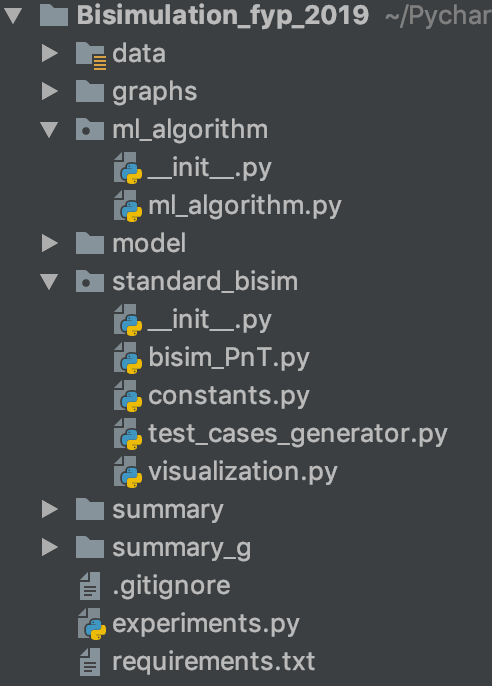
\includegraphics[width=0.4\textwidth]{img/actual_str.png}
    \caption{Actual structure}
    \label{fig:actual_str}
\end{figure}

\begin{description}
    \item[\texttt{/data/}] It is used to store the generated test cases data. They are saved as \texttt{.csv} file and are the output of \texttt{test\char`_cases\char`_generator.py}, the input of \texttt{ml\char`_algorithm.py}.
    
    \item[\texttt{/model/}] This directory is used to store the parameters of trained/half-trained machine learning models. It allowed training resume form break point and also directly apply of trained models.
    Models are save as \texttt{.ckpt} files.
    And during the training, \texttt{ml\char`_algorithm.py} will keep recording the current model.
    
    \item[\texttt{/graphs/}] The graphs figure that been visualised is put in this directory. 
    
    \item[\texttt{/summary/}] It is used to store the summary file generate by \texttt{ml\char`_algorithm.py}. These file record all the metric calculated during the training (i.e. loss, accuracy, precision and recall) for later analyse.
    
    \item[\texttt{/summary\char`_g/}] TensorFlow Graphs generated during the calculation of train are stored here. It can be visualised by the TensorBoard, which will do a great help in the implementation of the neural network.
    
    \item[\texttt{/requirement.txt}] This file is a text file which records all the package needed. An environment can be established easily based on this file.
    
    \item[\texttt{/.gitignore}] The project is managed by the distributed version control system \texttt{Git}. It is a configuration file that will make \texttt{Git} ignore assigned files.
    
    \item[\texttt{/experiments.py}] This file contain the experiments of the proeject, and will described in Section \ref{sec:experiment}.
    
    \item[\texttt{/standard\char`_bisim/}] Under this directory, that are \texttt{bisim\char`_PnT.py}, \texttt{test\char`_cases\char`_generator.py} and \texttt{visualisation.py}. Detail will described below (i.e. Section \ref{sec:comp_imp}). 
    
    \item[\texttt{/ml\char`_algorithm/}] It is used to hold \texttt{ml\char`_algorithm.py}. Detial of this part will be descussed below (i.e. Section \ref{sec:comp_imp}).
    
\end{description}


\subsection{Components Implementation}
\label{sec:comp_imp}
The detailed description of implementation is given in this part.

\subsubsection{Implementation of Standard Bisimulation Algorithm}
The first part of the project is to develop the standard bisimulation algorithm base on the algorithm given in \cite{Paige1987}.
This algorithm is implemented as a class \texttt{BisimPnT}.
Following functions are included.
Also the code listing of \texttt{coarsest\char`_partition() } is given here (See Listing \ref{lst:coarsest part}).\vspace{0.5em}

% \noindent
\begin{center}
\begin{tabularx}{0.9\textwidth}{lX}
    \toprule
    \textbf{Signature}          & \texttt{\char`_\char`_init\char`_\char`_(self, labels, graph\char`_g, graph\char`_h=None)}\\ \midrule
    \textbf{Description}        & Initiate the object. Union the given graphs and record the possible edges (\texttt{labels})\\ \midrule
    \textbf{Return}             & N/A \\ \bottomrule
\end{tabularx}
\end{center}
\begin{center}
\begin{tabularx}{0.9\textwidth}{lX}
    \toprule
    \textbf{Signature}          & \texttt{preimage(self, block\char`_s, label=None)}\\ \midrule
    \textbf{Description}        & Calculate the preimage of block with respect to a given type of edge (also relation). If type asigned, it will compute the preimage without distinguishing the types of edge, i.e. all edges will be seen as same relation (\texttt{label}).\\ \midrule
    \textbf{Return}             & $E^{-1}_{\text{label}}(\text{block\_s})=\{x|\exists y \in \text{block\_b } \text{such that } xE_\text{label}y\}$ \\ \bottomrule
\end{tabularx}
\end{center}
\begin{center}
\begin{tabularx}{0.9\textwidth}{lX}
    \toprule
    \textbf{Signature}          & \texttt{split\char`_block(self, block\char`_b, block\char`_s, label=None)}\\ \midrule
    \textbf{Description}        & Calculate the result of split the \texttt{block\char`_b} with the preimage of \texttt{block\char`_s}. It \texttt{label} is not assigned, then block b will be split with respect to all relation.\\ \midrule
    \textbf{Return}             & $\text{split}(\text{block\_b}, \text{block\_s}) = \{\text{block\_b}\cap E^{-1}_{\text{label}}(\text{block\_s}), \text{block\_b} - E^{-1}_{\text{label}}(\text{block\_s})\}$ \\ \bottomrule
\end{tabularx}
\end{center}
\begin{center}
\begin{tabularx}{0.9\textwidth}{lX}
    \toprule
    \textbf{Signature}          & \texttt{compound\char`_blocks(self, partition\char`_Q, partition\char`_X)}\\ \midrule
    \textbf{Description}        & Check if all the blocks in \texttt{parition\char`_X}, if their are compound or not. Return a set of all compound blocks. \\ \midrule
    \textbf{Return}             & a set of blocks in \texttt{partition\char`_X} that is compound with respect to \texttt{partition\char`_Q} \\ \bottomrule
\end{tabularx}
\end{center}
\begin{center}
\begin{tabularx}{0.9\textwidth}{lX}
    \toprule
    \textbf{Signature}          & \texttt{is\char`_compound\char`_to(self, block\char`_s, partition)}\\ \midrule
    \textbf{Description}        & Check if \texttt{block\char`_s} is compound with respect to \texttt{partition}, i.e. if \texttt{block\char`_s} contain more then one block in \texttt{partition}. \\ \midrule
    \textbf{Return}             & The smaller contained block in \texttt{partition} of \texttt{False} if \texttt{block\char`_s} is simple \\ \bottomrule
\end{tabularx}
\end{center}
\begin{center}
\begin{tabularx}{0.9\textwidth}{lX}
    \toprule
    \textbf{Signature}          & \texttt{coarsest\char`_partition(self, plot=False)}\\ \midrule
    \textbf{Description}        & Calculate the coarsest partition of the graph given when initialisation. \\ \midrule
    \textbf{Return}             & The coarsest partition \\ \bottomrule
\end{tabularx}
\end{center}
\begin{center}
\begin{tabularx}{0.9\textwidth}{lX}
    \toprule
    \textbf{Signature}          & \texttt{get\char`_min\char`_graph(self)}\\ \midrule
    \textbf{Description}        & Assemble a min bisimulation graph.  \\ \midrule
    \textbf{Return}             & The minimum bisimulation graph\\ \bottomrule
\end{tabularx}
\end{center}
\begin{center}
\begin{tabularx}{0.9\textwidth}{lX}
    \toprule
    \textbf{Signature}          & \texttt{is\char`_bisimilar(self)}\\ \midrule
    \textbf{Description}        & Check it two given graph is bisimulation by checking if there are nodes from both graph in each of the coarsest partition. \\ \midrule
    \textbf{Return}             & \texttt{True} or \texttt{False}\\ \bottomrule
\end{tabularx}
\end{center}

% \captionof{listing}{Function calculate coarsest partition \label{lst:coarsest part}}\vspace{-0.6em}
\begin{code}
\caption{Function calculate coarsest partition}
\label{lst:coarsest part}
\begin{minted}[linenos, frame=single,breaklines]{python}
def coarsest_partition(self, plot=False):

    # Step 1 Initial U 
    block_u = set(self.full_graph_U.nodes())
    
    # Step 2
    partition_X = [block_u]
    block_set_C = [block_u]
    
    # Step 3
    partition_Q = self.split_block(block_u, block_u)
    
    # Step 4
    block_set_C = self.compound_blocks(partition_Q, partition_X)
    while len(block_set_C) != 0:
        # Step a:
        # select refining block_b
        # a compound block of partition_X
        block_s = block_set_C.pop()  
        # a block of Q that contained in s
        block_b = self.is_compound_to(block_s, partition_Q)  

        # Step c:
        # update X:
        partition_X.remove(block_s)
        partition_X.append(block_s - block_b)
        partition_X.append(block_b)  # split block S in X

        # if the rest is still not simple, put it back to C
        if self.is_compound_to(block_s - block_b, partition_Q) is not False:
            block_set_C.append(block_s)
        
        # Step d
        for label in self.labels:

            # compute preimage of B
            preimage_b = self.preimage(block_b, label)
            # compute preimage of S - B
            preimage_s_sub_b = self.preimage(block_s - block_b, label)

            # refine Q with respect to B and S-B
            new_partition_Q = []
            for block_d in partition_Q:
                block_d1 = block_d.intersection(preimage_b)
                block_d2 = block_d - block_d1
                block_d11 = block_d1.intersection(preimage_s_sub_b)
                block_d12 = block_d1 - preimage_s_sub_b

                if len(block_d2) and block_d2 not in new_partition_Q:
                    new_partition_Q.append(block_d2)
                if len(block_d11) and block_d11 not in new_partition_Q:
                    new_partition_Q.append(block_d11)
                if len(block_d12) and block_d12 not in new_partition_Q:
                    new_partition_Q.append(block_d12)
                partition_Q = new_partition_Q
        
        # Step 5
        block_set_C = self.compound_blocks(partition_Q, partition_X)
        # if needed visualise the result
        if plot:
            vi.plot_graph_with_partition(self.full_graph_U, partition_Q)

    self.co_partition = partition_Q
    return partition_Q
\end{minted}
\end{code}


However, there is a visualisation tool that can plot the multi-directed graphs (e.g. Figure \ref{fig:example1_model} is drawn by this tool) are developed based on \texttt{graphviz}. 
It can also colour the graph with a given partition.

With this tool, the development and component tests became much easier.
There is one main function below.
\begin{center}
\begin{tabularx}{0.9\textwidth}{lX}
    \toprule
    \textbf{Signature}          & \texttt{plot\char`_graph\char`_with\char`_partition(graph, blocks=None, file\char`_name="test")}\\ \midrule
    \textbf{Description}        & Visualisation the graph with partition and save the image. If no \texttt{blocks} (i.e. partition) given it will output image without colour.\\ \midrule
    \textbf{Return}             & Image file \\ \bottomrule
\end{tabularx}
\end{center}


\subsubsection{Implementation of Test Case Generator}\label{sec:imptestcasegenerator}
It was considered that there are two generators (see Section \ref{sec:generator ds}).
However, during the primary test, the full test generator (see Algorithm \ref{alg:F_tcg}) is too expensive both in computation and space.
Specifically, for the graphs with $n$ node and $m$ types of edges.
Then there are $2^{n*n*m}$ possible graphs.
After combination, there will be $(2^{n^2m}*(2^{n^2m}-1))/2 \approx 2^{2n^2m}$.
If graphs have 3 nodes and 2 types of edges, there will be $2^{36}$ (around 60 billion) test cases.
Thus, it is too expensive for this project.
Instead, we will repeat the experiments in different parameters to minimise the possibles.

Here we give the code about random test case generator described in Algorithm \ref{alg:R_tcg} and the heuristic algorithm for generate bisimilar graph (see Algorithm \ref{alg:R_tcg}, Step \ref{item:bi} to Step \ref{item:bi_end}).
Also, the generator is packed as a command line tool for the convenience of further use (see Figure \ref{fig:arggenerator}).
\begin{figure}[h]
    \centering
    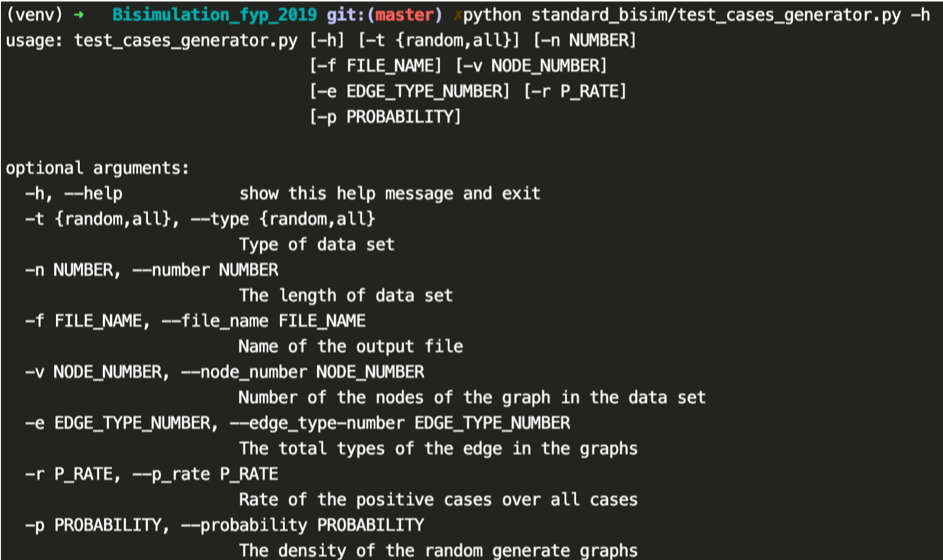
\includegraphics[width=0.9\textwidth]{img/generator.png}
    \caption{Arguments of test cases generator}
    \label{fig:arggenerator}
\end{figure}

% \captionof{listing}{Random test case generator \label{lst:ramgene}}\vspace{-0.6em}
\begin{code}
\caption{Random test case generator}
\label{lst:ramgene}
\begin{minted}[linenos, frame=single,breaklines]{python}
def test_cases_generator(c_type="random", number=100, file_name="test_cases", min_node_number=5, edge_type_number=3, probability=0.5, p_rate=0.5):
    labels = [chr(97 + i) for i in xrange(edge_type_number)]
    if not os.access('./data/', os.R_OK):
        os.mkdir('./data/')
    with open('./data/' + file_name + '.csv', 'w') as csvfile:
        print('write in path: ' + './data/' + file_name + '.csv')
        if c_type == 'random':
            fieldnames = ['g1', 'g2', 'bis']
            writer = csv.DictWriter(csvfile, fieldnames=fieldnames)
            writer.writeheader()

            for _ in xrange(number):
                if _ % (number/10) == 0: print("generating # %d" % _)
                g1 = ''
                while not g1 or not nx.is_weakly_connected(g1):
                    g1 = random_labeled_digraph(min_node_number, edge_type_number, random.random() * probability)
                g1_bin = get_bin_array_from_graph(g1, min_node_number, edge_type_number)
                bis = 1
                if random.random() > p_rate:
                    g2 = generate_random_similar(g1, edge_type_number)
                else:
                    g2 = random_labeled_digraph(min_node_number, edge_type_number, random.random() * probability)
                    k = bi.BisimPnT(labels, g1, g2)
                    bis = int(k.is_bisimilar())
                g2_bin = get_bin_array_from_graph(g2, min_node_number, edge_type_number)
                writer.writerow({fieldnames[0]: g1_bin, fieldnames[1]: g2_bin, fieldnames[2]: bis})
\end{minted}
\end{code}

% \captionof{listing}{Function of generating random bisimilar graph \label{lst:genrdmsim}}\vspace{-0.6em}
\begin{code}
\caption{Function of generating random bisimilar graph}
\label{lst:genrdmsim}
\begin{minted}[linenos, frame=single,breaklines]{python}
def generate_random_similar(graph, edge_type_number):
    k = bi.BisimPnT([chr(97 + t) for t in range(edge_type_number)], graph)
    min_graph = k.get_min_graph()
    min_node_number = min_graph.order()
    partition = [{i} for i in range(min_node_number)]
    node_number = graph.order()
    if min_node_number == node_number:
        return random_relabel_nodes(graph)
    for i in xrange(min_node_number, node_number):
        partition[random.randint(0, min_node_number - 1)].add(i)
    result_graph = None
    # print min_node_number, node_number
    while not result_graph or result_graph.order() != graph.order():
        result_graph = nx.MultiDiGraph()
        for start_node_type in xrange(min_node_number):
            for end_node_type in min_graph.successors(start_node_type):  # for each origin type pair
                for edge_label in {edge['label'] for edge in min_graph.get_edge_data(start_node_type, end_node_type).values()}:
                    # for each type edge
                    accept = False
                    while not accept:
                        start_nodes = random.sample(partition[start_node_type], random.randint(0, len(partition[start_node_type])))
                        for start_node in start_nodes:
                            end_nodes = random.sample(partition[end_node_type], random.randint(0, len(partition[end_node_type])))
                            for end_node in end_nodes:
                                exist_types = {exist_type_dic['label'] for exist_type_dic in result_graph.get_edge_data( start_node,end_node, default={0:{'label':'#'}}).values()}
                                if  edge_label not in exist_types:
                                    result_graph.add_edge(start_node, end_node, label=edge_label)
                        t1 = partition[start_node_type].copy()
                        t2 = partition[end_node_type].copy()
                        for start_node in partition[start_node_type]:
                            for end_node in partition[end_node_type]:
                                exist_types = {exist_type_dic['label'] for exist_type_dic in result_graph.get_edge_data( start_node,end_node, default={0:{'label':'#'}}).values()}
                                if edge_label in exist_types:
                                    t1.discard(start_node)
                                    t2.discard(end_node)
                        accept = not bool(t1) and not bool(t2)
    return result_graph
\end{minted}
\end{code}


\subsubsection{Implementation of Machine Learning}
This neural network is developed on the \texttt{Tensorflow} along with the visualisation tool \texttt{TensorBoard}.
TensorFlow Graph is a computation graph drew by \texttt{TensorBoard} that indicates the process of the computation.
Figure \ref{fig:tfgraph} are the TensorFlow graph of the network model .

After all parameters are randomly initialised by \texttt{tf.random\char`_normal\char`_initialiser()}, the model start with a fixed length ($mn^2$) input layer, and accept the numeral input, i.e. the 1 or 0 in the adjacency matrix are accepted as a number rather than a catalogue.
And the activate function used here is rectified linear unite (ReLU).
Because it is computationally efficient and more plausible on biology which may improve the comprehension of the model.
Also it promises fewer problems on vanishing gradient \cite{pmlr-v15-glorot11a}.
The adjacency matrixes become tensor after input.
Then the tensor of each graph goes through the re-representing part (see g1\_p and g2\_p in Figure \ref{fig:tfgraph}).
After that, they are merged into one big tensor and go through the distinguishing part (see merge and logits in Figure \ref{fig:tfgraph}).
At the end of the distinguishing part, the tensor is output as logits, i.e. two number that indicated the possibility of bisimilar or not.
Finally pass through a \emph{softmax} layer the prediction will be given.
Yet, during the training, there are metrics including loss, accuracy, precision, recall logged for further studying.
The main code is shown in Listing \ref{lst:mlat}.
It is also packed as a commend line tools (see Figure \ref{fig:argmlal}).

\begin{figure}[h]
\centering
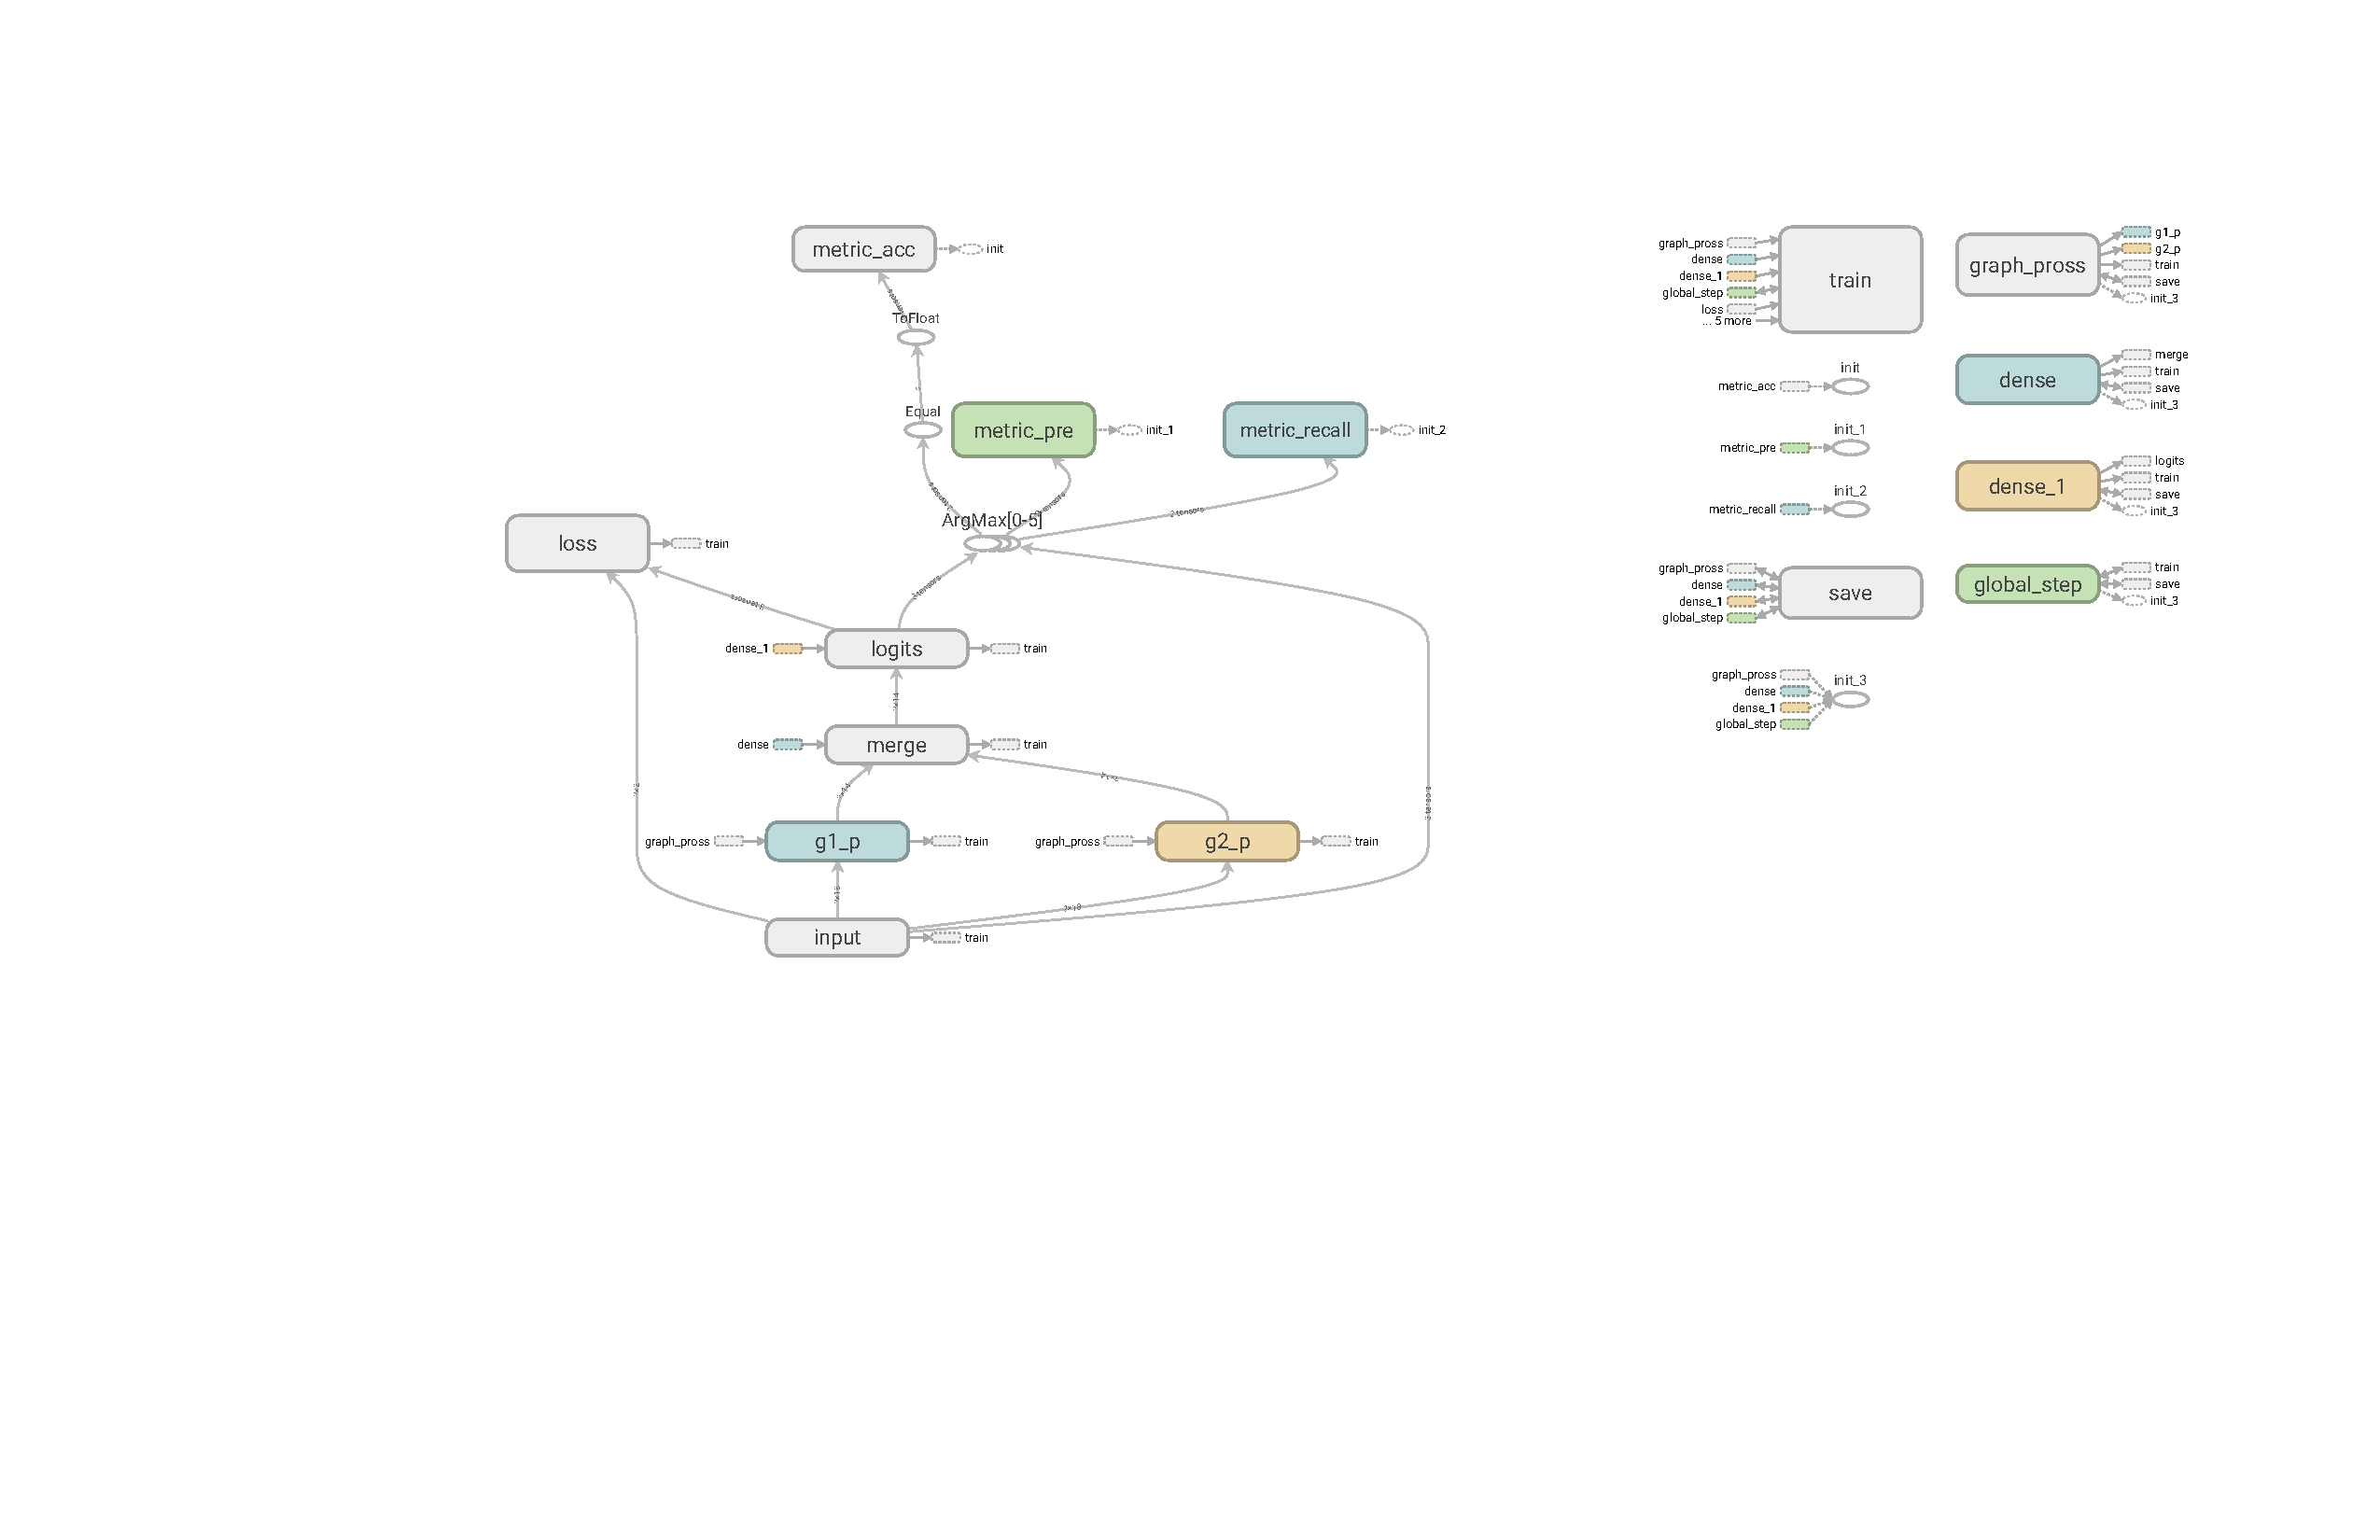
\includegraphics[width=\textwidth]{img/tfgraph.pdf}
\caption{TensorFlow graph of MLP}
\label{fig:tfgraph}
\end{figure}

\begin{figure}[h]
    \centering
    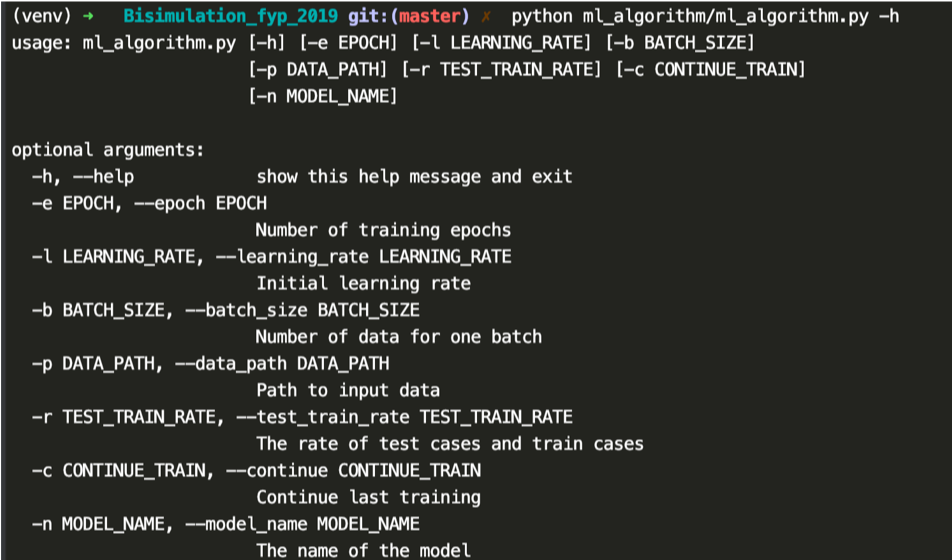
\includegraphics[width=0.9\textwidth]{img/mlalgorithm.png}
    \caption{Arguments of machine learning algorithm}
    \label{fig:argmlal}
\end{figure}


% \captionof{listing}{ML algorithm and training \label{lst:mlat}}\vspace{-0.6em}
\begin{code}
\caption{ML algorithm and training}
\label{lst:mlat}
\begin{minted}[linenos, frame=single,breaklines]{python}
def fc(self, continue_train=False):

    kernel_initializer = tf.initializers.glorot_normal()
    tf.reset_default_graph()
    small_layer_number = int(math.log(self.tupe_length) * 5)
    # print small_layer_number, self.tupe_length
    with tf.name_scope('input'):
        g1 = tf.placeholder(tf.float32, [None, self.tupe_length])
        g2 = tf.placeholder(tf.float32, [None, self.tupe_length])
        y = tf.placeholder(tf.float32, [None, 2])

    with tf.name_scope('g1_p'):
        with tf.variable_scope('graph_pross'):
            g1_dence1 = tf.layers.dense(g1, self.tupe_length, activation=tf.nn.relu, kernel_initializer=kernel_initializer, bias_initializer=tf.random_normal_initializer(), name='dence1')

            g1_s_dence1 = tf.layers.dense(g1_dence1, small_layer_number, activation=tf.nn.relu, kernel_initializer=kernel_initializer, bias_initializer=tf.random_normal_initializer(), name='s_dence1')

    with tf.name_scope('g2_p'):
        with tf.variable_scope('graph_pross', reuse=True):
            g2_dence1 = tf.layers.dense(g2, self.tupe_length, activation=tf.nn.relu, name='dence1', reuse=True)

            g2_s_dence1 = tf.layers.dense(g2_dence1, small_layer_number, activation=tf.nn.relu, name='s_dence1', reuse=True)
    with tf.name_scope('merge'):
        two_graphs = tf.concat([g1_s_dence1, g2_s_dence1], 1)
        merge_layer = tf.layers.dense(two_graphs, small_layer_number, activation=tf.nn.relu, kernel_initializer=kernel_initializer, bias_initializer=tf.random_normal_initializer())
    with tf.name_scope('logits'):
        logits = tf.layers.dense(merge_layer, 2, activation=tf.identity, kernel_initializer=kernel_initializer, bias_initializer=tf.random_normal_initializer())
    with tf.name_scope('loss'):
        loss = tf.losses.softmax_cross_entropy(y, logits)
        tf.summary.scalar('loss', loss)

    global_step = tf.Variable(0, trainable=False, name='global_step')

    with tf.name_scope('train'):
        train = tf.train.AdadeltaOptimizer(learning_rate=self.learning_rate) .minimize(loss=loss, global_step=global_step)

    acc_metric, acc_metric_update = tf.metrics.accuracy(tf.argmax(logits, 1), tf.argmax(y, 1), name='metric_acc')
    pre_metric, pre_metric_update = tf.metrics.precision(tf.argmax(logits, 1), tf.argmax(y, 1), name='metric_pre')
    recall_metric, recall_metric_update = tf.metrics.recall(tf.argmax(logits, 1), tf.argmax(y, 1), name='metric_recall')
    tf.summary.scalar('accuracy', acc_metric_update)
    tf.summary.scalar('precision', pre_metric_update)
    tf.summary.scalar('recall', recall_metric_update)

    metric_acc_var = tf.get_collection(tf.GraphKeys.LOCAL_VARIABLES, scope="metric_acc")
    acc_initializer = tf.variables_initializer(var_list=metric_acc_var)
    metric_pre_var = tf.get_collection(tf.GraphKeys.LOCAL_VARIABLES, scope="metric_pre")
    pre_initializer = tf.variables_initializer(var_list=metric_pre_var)
    metric_recall_var = tf.get_collection(tf.GraphKeys.LOCAL_VARIABLES, scope="metric_recall")
    recall_initializer = tf.variables_initializer(var_list=metric_recall_var)

    merged_summary = tf.summary.merge_all()
    saver = tf.train.Saver()

    with tf.Session() as sess:
        if continue_train:
            saver.restore(sess, DIR_MODEL + '/' + self.model_name + '/model.ckpt')
            print('continue training, model loaded')
        else:
            self.clean_old_record()
            print('new training, old record cleaned')
            # initial
            sess.run(tf.global_variables_initializer())

        train_writer = tf.summary.FileWriter(DIR_SUMMARY + '/' + self.model_name, sess.graph)
        test_writer = tf.summary.FileWriter(DIR_SUMMARY + '/' + self.model_name + '_test')

        for epoch in range(self.epochs):
            sess.run([acc_initializer, pre_initializer, recall_initializer])
            loss_p = None
            g_step = None

            summary_11, g_step_1= sess.run([merged_summary,global_step], feed_dict={g1: self.g1_dfs[1], g2: self.g2_dfs[1], y: self.label_dfs[1]})

            test_writer.add_summary(summary_11, g_step_1)

            for i in range(self.batch_number):
                _, loss_p, summary, g_step = sess.run([train, loss, merged_summary, global_step], feed_dict={g1: self.g1_dfs[0][i], g2: self.g2_dfs[0][i], y: self.label_dfs[0][i]})
                train_writer.add_summary(summary, g_step)

            if epoch % 10 == 0:
                # summary,acc = sess.run([merged_summary ,acc_metric])
                acc, pre, recall = sess.run([acc_metric, pre_metric, recall_metric])
                log_str = "Epoch %d \t G_step %d \t Loss=%f \t Accuracy=%f \t Precision=%f \t Recall=%f "
                print(log_str % (epoch, g_step, loss_p, acc, pre, recall))
                saver.save(sess, DIR_MODEL + '/' + self.model_name + '/model.ckpt')

    train_writer.close()
    test_writer.close()
\end{minted}
\end{code}


\newpage
\subsection{Components Test}
\label{sec:comptest}
During the development, some tests are used for examining each component.
Here some of the test cases and the test results will be given.

\subsubsection{Test for Standard Bisimulation Algorithm}
The test cases used here is from the textbook.
And by manipulating these cases, this component can be tested.

\vspace{+0.2em}
\noindent\textbf{Test case 1:}

\noindent This case is form \cite{Stirling2011a}. 
By changing two egdes in this case (i.e. $\text{H-4}\stackrel{b}{\rightarrow}\text{H-5} \Longrightarrow \text{H-4}\stackrel{c}{\rightarrow}\text{H-5}$, $\text{G-2}\stackrel{b}{\rightarrow}\text{G-4} \Longrightarrow \text{G-2}\stackrel{c}{\rightarrow}\text{G-4}$), these two graph should lose bisimulation equivalence.
The test code is shown in Listing \ref{lst:test1}.
The output is shown in Figure \ref{fig:output1}-\ref{fig:output1g-}.
Notice that in a figure like Figure \ref{fig:output1g}, edges that are one type has the same colour and nodes in the same partition (i.e. are bisimilar) will be painted in the same colour.
% \captionof{listing}{Test code for case 1 \label{lst:test1}}
% \vspace{-0.5em}
\begin{code}
\caption{Test code for case 1}
\label{lst:test1}
\begin{minted}[linenos, frame=single,breaklines]{python}
# =============== example 1 ===============
G = nx.MultiDiGraph()
G.add_edge(5, 2, label='a')
G.add_edge(2, 3, label='b')
G.add_edge(2, 4, label='b')
# G.add_edge(2, 4, label='c')

H = nx.MultiDiGraph()
H.add_edge(1, 2, label='a')
H.add_edge(1, 4, label='a')
H.add_edge(2, 3, label='b')
H.add_edge(4, 5, label='b')
# H.add_edge(4, 5, label='c')

labels = ['a', 'b']
# labels = ['a', 'b', 'c']

k = BisimPnT(labels, G, H)
par = k.coarsest_partition()
vi.plot_graph_with_partition(k.full_graph_U,par,'example_1')
vi.plot_graph(BisimPnT(labels,H).get_min_graph(), 'mini_g')
print("Example 1: ")
print(par)
print(k.is_bisimilar())
\end{minted}
\end{code}

\begin{figure}[H]
\centering
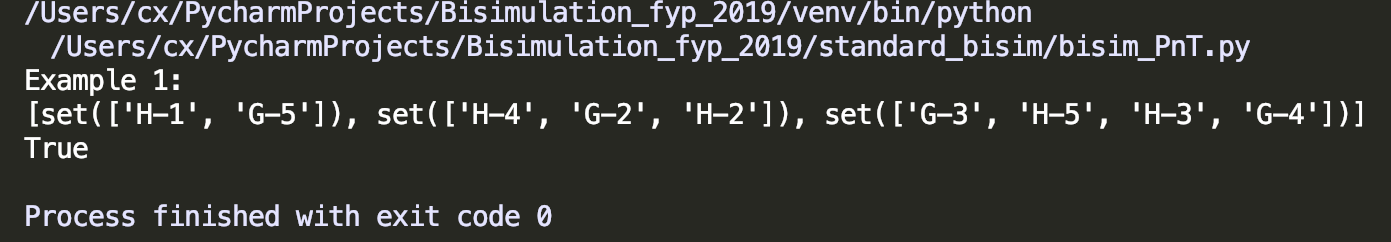
\includegraphics[width=0.9\textwidth]{img/output1.png}
\caption{Output for test case 1 positive instance}
\label{fig:output1}
\end{figure}

\begin{figure}[H]
    \centering
    \subfigure[Mini graph]{
        % \label{fig:example1_model}
        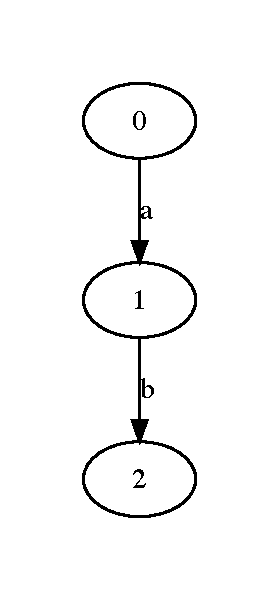
\includegraphics[height=16em]{img/output1min.pdf}}
    \subfigure[Coloured graphs]{
        % \label{fig:example1_matrix}
        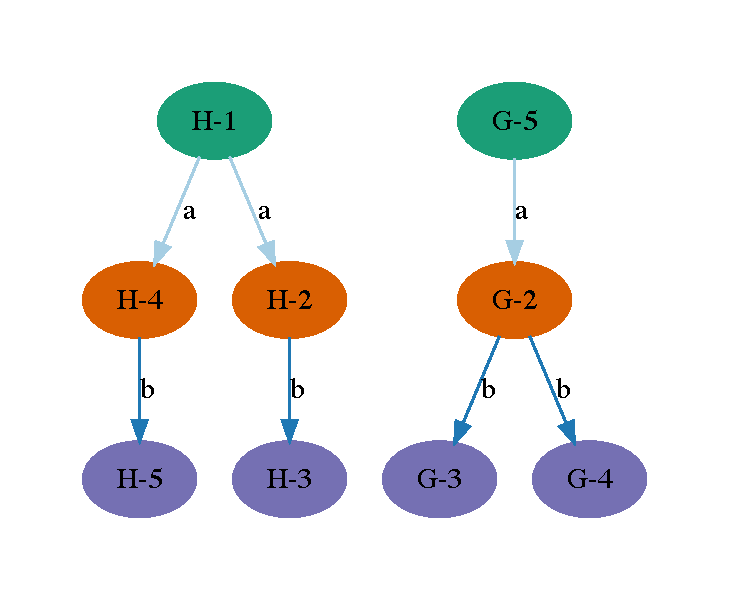
\includegraphics[height=16em]{img/output1g.pdf}}
    \caption{Test case 1: positive instance}
    \label{fig:output1g}
\end{figure}

\begin{figure}[H]
\centering
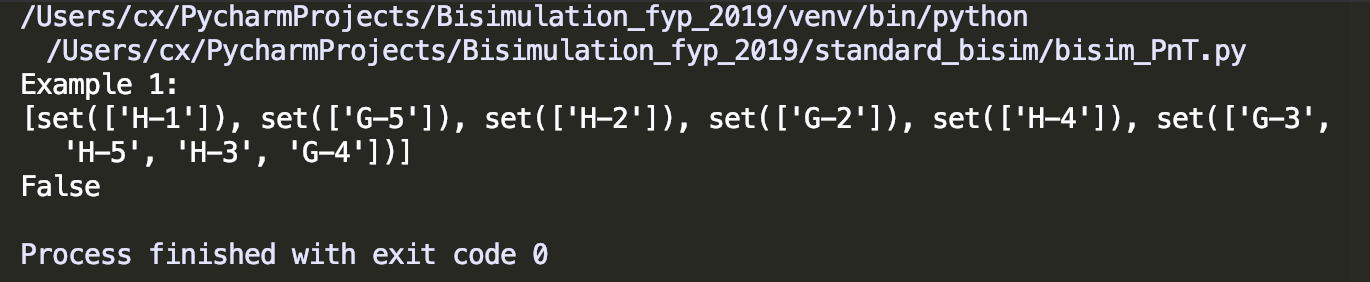
\includegraphics[width=0.9\textwidth]{img/output1-.png}
\caption{Output for test case 1 negative instance}
\label{fig:output1-}
\end{figure}

\begin{figure}[H]
    \centering
    % \label{fig:example1_matrix}
    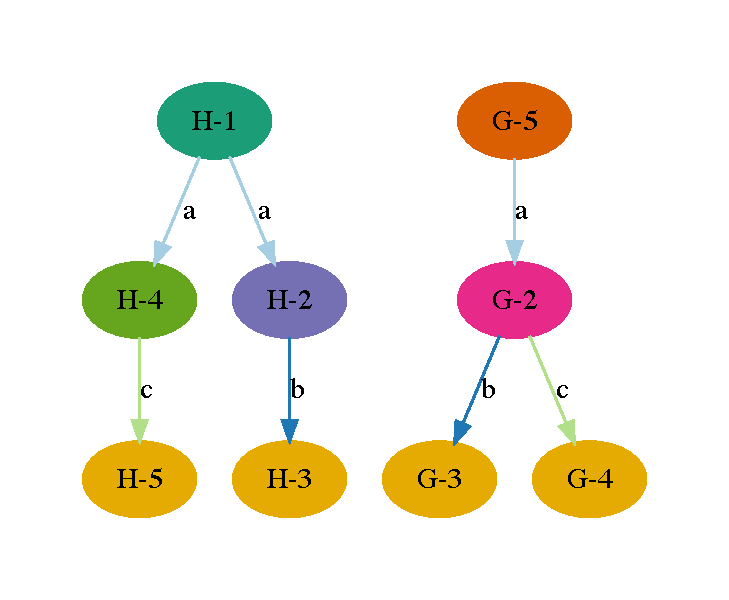
\includegraphics[height=16em]{img/output1g-.pdf}
    \caption{Test case 1: negative instance}
    \label{fig:output1g-}
\end{figure}

\vspace{+0.2em}
\noindent\textbf{Test case 2:}

\noindent This case is form \cite{Stirling2011a}.
By changing two egdes in this case (i.e. $\text{G-3}\stackrel{c}{\rightarrow}\text{G-2} \Longrightarrow \text{G-3}\stackrel{b}{\rightarrow}\text{G-2}$ these two graph should lose bisimulation equivalence.
The test code is shown in Listing \ref{lst:test2}.
The output of the test result is shown in Figure \ref{fig:output2}-\ref{fig:output2g-}.
% \captionof{listing}{Test code for case 2 \label{lst:test2}}\vspace{-0.5em}
\begin{code}
\caption{Test code for case 2}
\label{lst:test2}
\begin{minted}[linenos, frame=single,breaklines]{python}
# =============== example 2 ===============
G = nx.MultiDiGraph()
G.add_edge(1, 3, label='a')
G.add_edge(1, 2, label='a')
G.add_edge(2, 3, label='b')
G.add_edge(3, 1, label='c')
G.add_edge(3, 2, label='c')
# G.add_edge(3, 2, label='b')

H = nx.MultiDiGraph()
H.add_edge(1, 3, label='a')
H.add_edge(1, 4, label='a')
H.add_edge(2, 3, label='b')
H.add_edge(3, 1, label='c')
H.add_edge(3, 4, label='c')
H.add_edge(4, 5, label='b')
H.add_edge(5, 1, label='c')
H.add_edge(5, 2, label='c')

labels = ['a', 'b', 'c']
k = BisimPnT(labels, G, H)
partition = k.coarsest_partition()
vi.plot_graph_with_partition(k.full_graph_U, partition, 'example_2')
vi.plot_graph(BisimPnT(labels, H).get_min_graph(), 'mini_g2')
print("Example 2: ")
print(partition)
print(k.is_bisimilar())
\end{minted}
\end{code}

\begin{figure}[H]
\centering
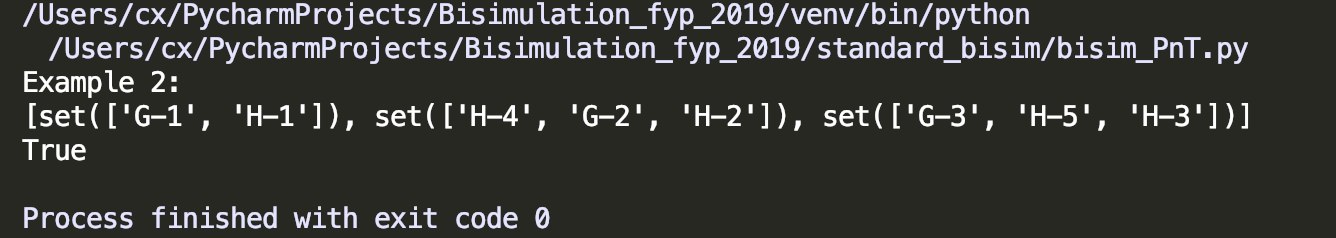
\includegraphics[width=0.9\textwidth]{img/output2.png}
\caption{Output for test case 2 positive instance}
\label{fig:output2}
\end{figure}

\begin{figure}[H]
    \centering
    \subfigure[Mini graph]{
        % \label{fig:example1_model}
        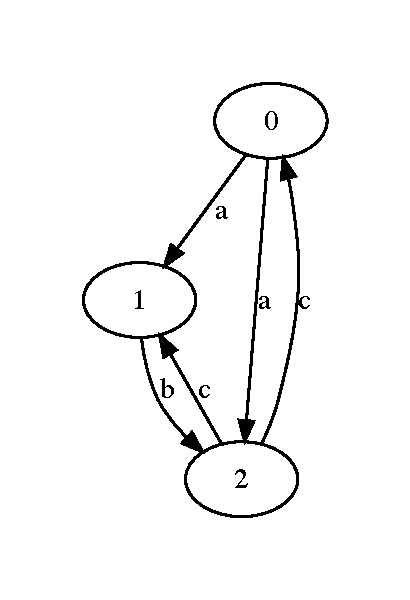
\includegraphics[height=14em]{img/output2min.pdf}}
    \subfigure[Coloured graphs]{
        % \label{fig:example1_matrix}
        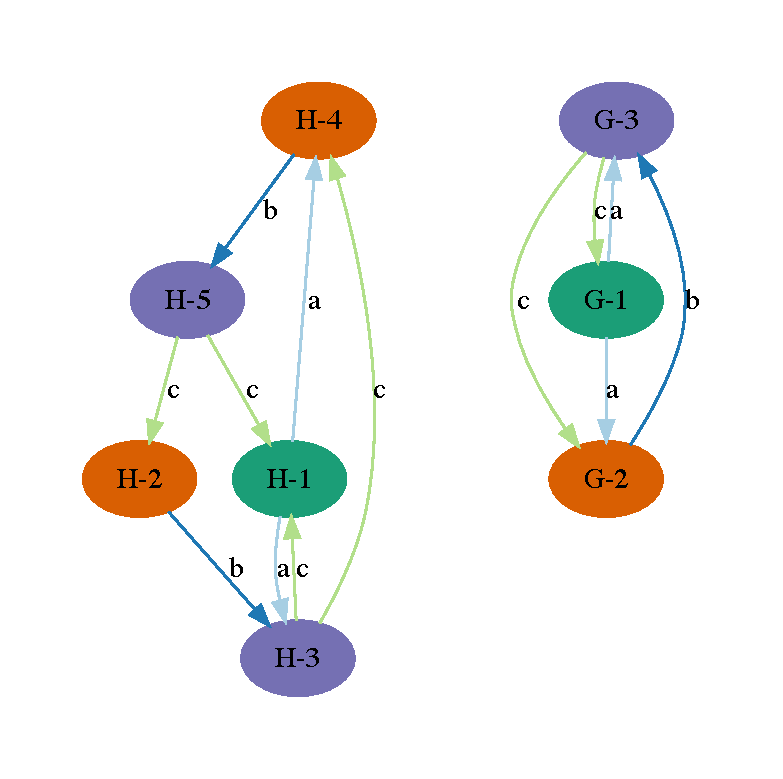
\includegraphics[height=16em]{img/output2g.pdf}}
    \caption{Test case 2: positive instance}
    \label{fig:output2g}
\end{figure}

\begin{figure}[H]
\centering
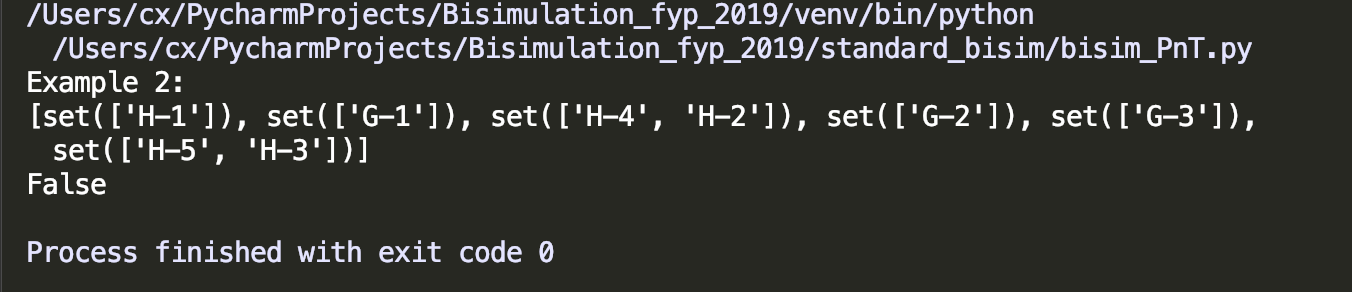
\includegraphics[width=0.9\textwidth]{img/output2-.png}
\caption{Output for test case 1 negative instance}
\label{fig:output2-}
\end{figure}
\begin{figure}[H]
    \centering
    % \label{fig:example1_matrix}
    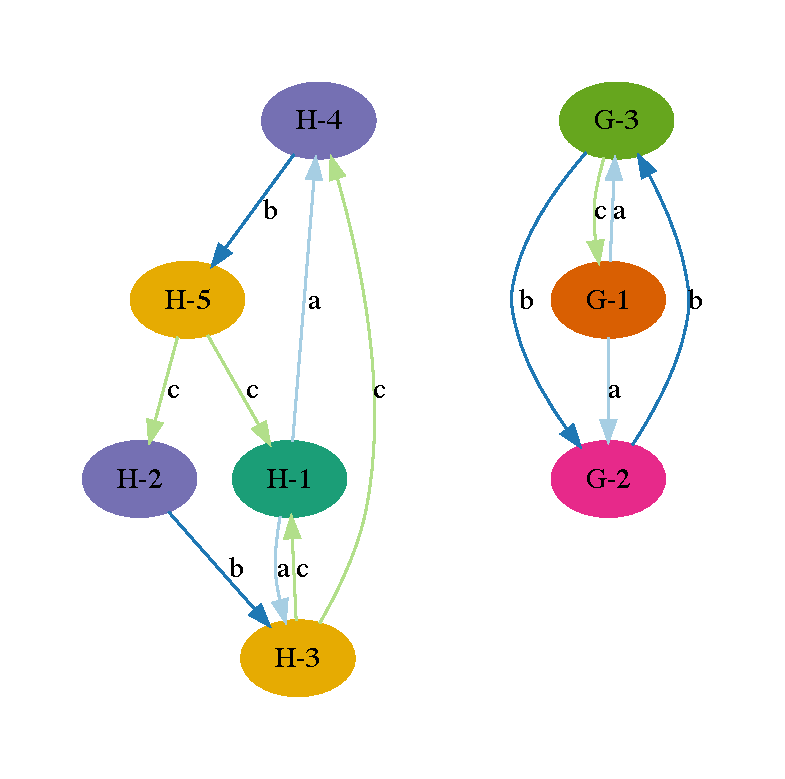
\includegraphics[height=16em]{img/output2g-.pdf}
    \caption{Test case 2: negative instance}
    \label{fig:output2g-}
\end{figure}

\subsubsection{Test for test case generator}

\textbf{Function for Generating Random bisimilar Graph:}

\noindent Firstly the function \texttt{generate\char`_random\char`_similar()} is tested.
The idea of testing is to randomly generate a graph then call the function.
Use the \emph{standard bisimulation algorithm} to compute the bisimulation equivalence of the output (to be seen in Listing \ref{lst:testg}).
Here, we also give some test generated results (see Figure \ref{fig:outputg1}-\ref{fig:outputg4}).
Notice that these results are selected examples for different types of result.


% \captionof{listing}{Test code for \texttt{generate\char`_random\char`_similar} \label{lst:testg}}\vspace{-0.5em}
\begin{code}
\caption{Test code for \texttt{generate\char`_random\char`_similar}}
\label{lst:testg}
\begin{minted}[linenos, frame=single,breaklines]{python}
# =============== test for random_labeled_digraph() ===============
flag = True
i = 0

# if there are any error the loop will break
# until reach the test time
while flag :
    i = i+1
    a = random_labeled_digraph(5,2,0.5*random.random())
    b = generate_random_similar(a, 2)
    k = bi.BisimPnT(['a','b'],a,b)
    flag = k.is_bisimilar()
    print i
    print flag
    if i == 100:
        break

vi.plot_graph(a, 'test')
vi.plot_graph(bi.BisimPnT(['a','b'],a).get_min_graph(),"mini_a")
vi.plot_graph(b, 'test1')
vi.plot_graph(bi.BisimPnT(['a','b'],a).get_min_graph(),"mini_b")
\end{minted}
\end{code}


\begin{figure}[H]
    \centering
    \subfigure[Mini graph]{
        % \label{fig:example1_model}
        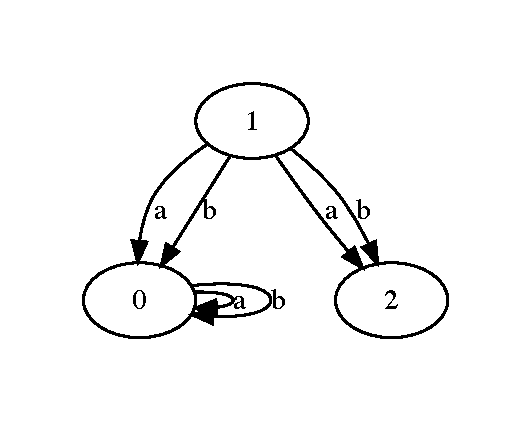
\includegraphics[height=9em]{img/outputg1m.pdf}}
    \subfigure[Coloured graphs]{
        % \label{fig:example1_matrix}
        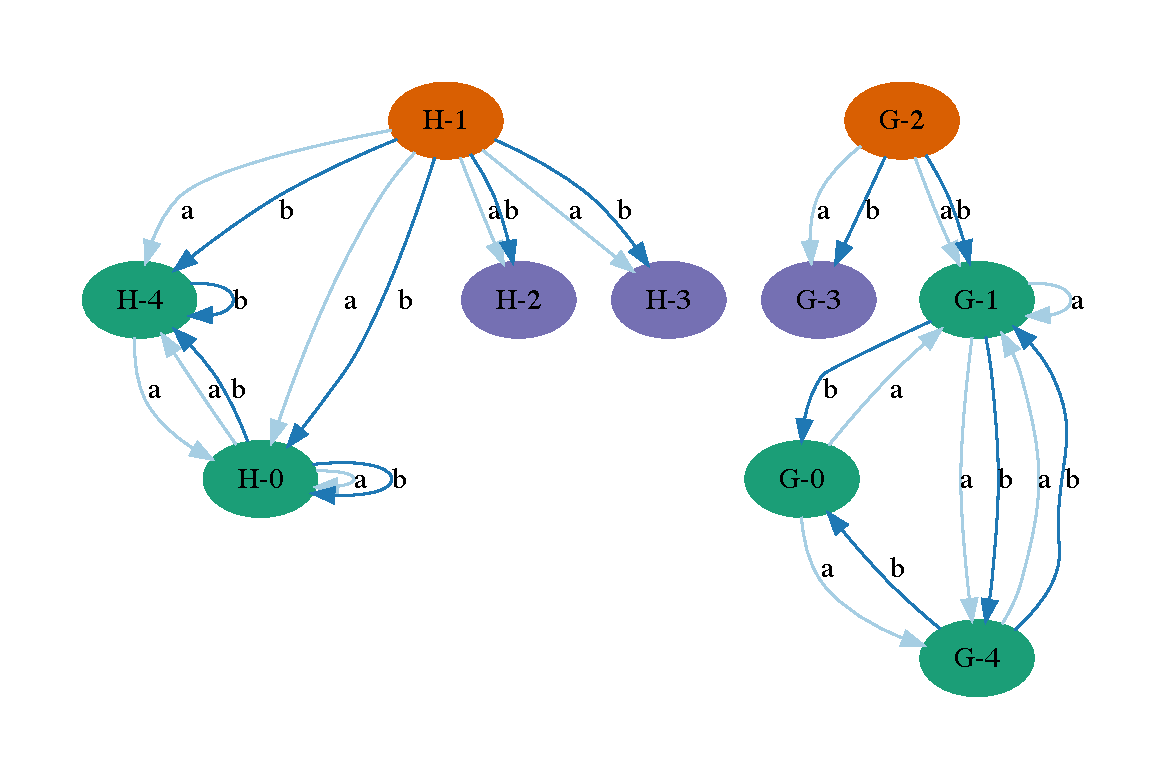
\includegraphics[height=17em]{img/outputg1.pdf}}
    \caption{Test result 1}
    \label{fig:outputg1}
\end{figure}

\begin{figure}[H]
    \centering
    \subfigure[Mini graph]{
        % \label{fig:example1_model}
        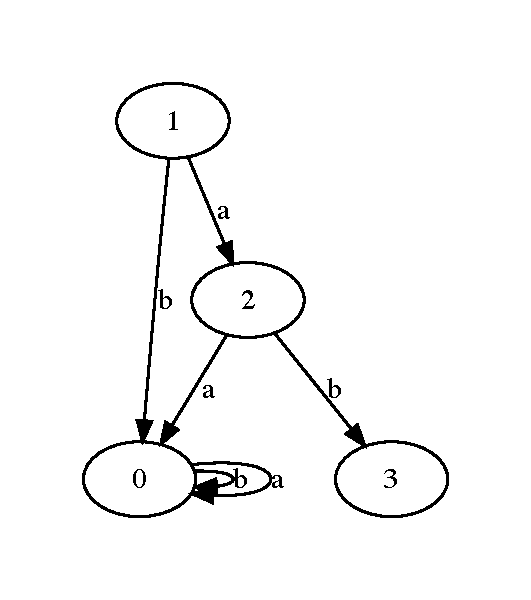
\includegraphics[height=12em]{img/outputg2m.pdf}}
    \subfigure[Coloured graphs]{
        % \label{fig:example1_matrix}
        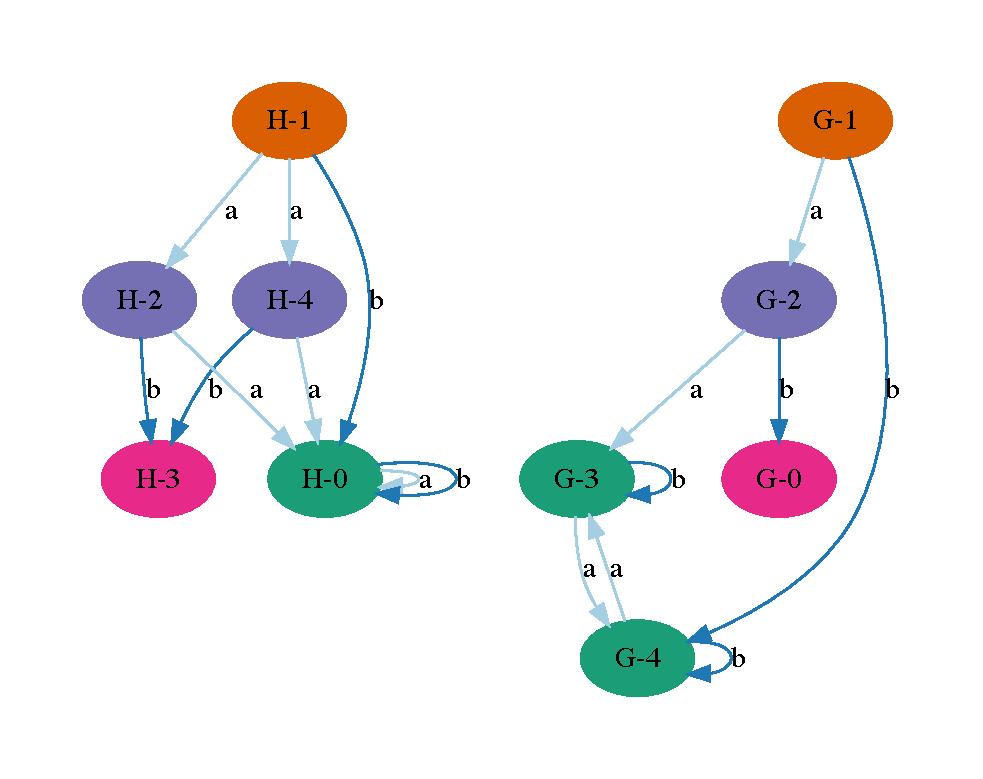
\includegraphics[height=17em]{img/outputg2.pdf}}
    \caption{Test result 2}
    \label{fig:outputg2}
\end{figure}

\begin{figure}[H]
    \centering
    \subfigure[Mini graph]{
        % \label{fig:example1_model}
        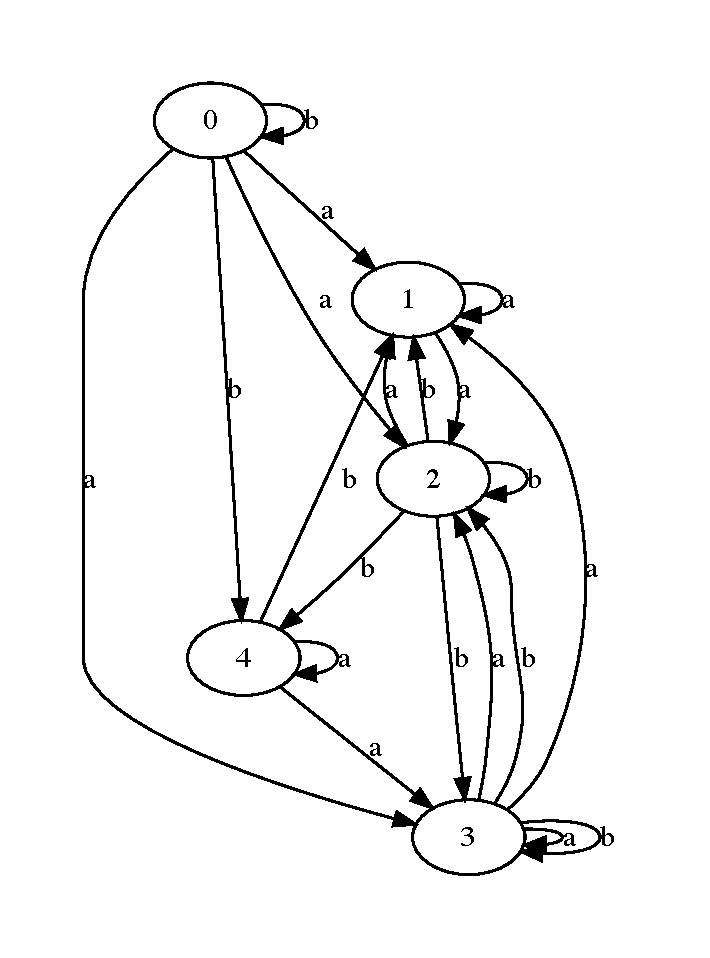
\includegraphics[height=15em]{img/outputg3m.pdf}}
    \subfigure[Coloured graphs]{
        % \label{fig:example1_matrix}
        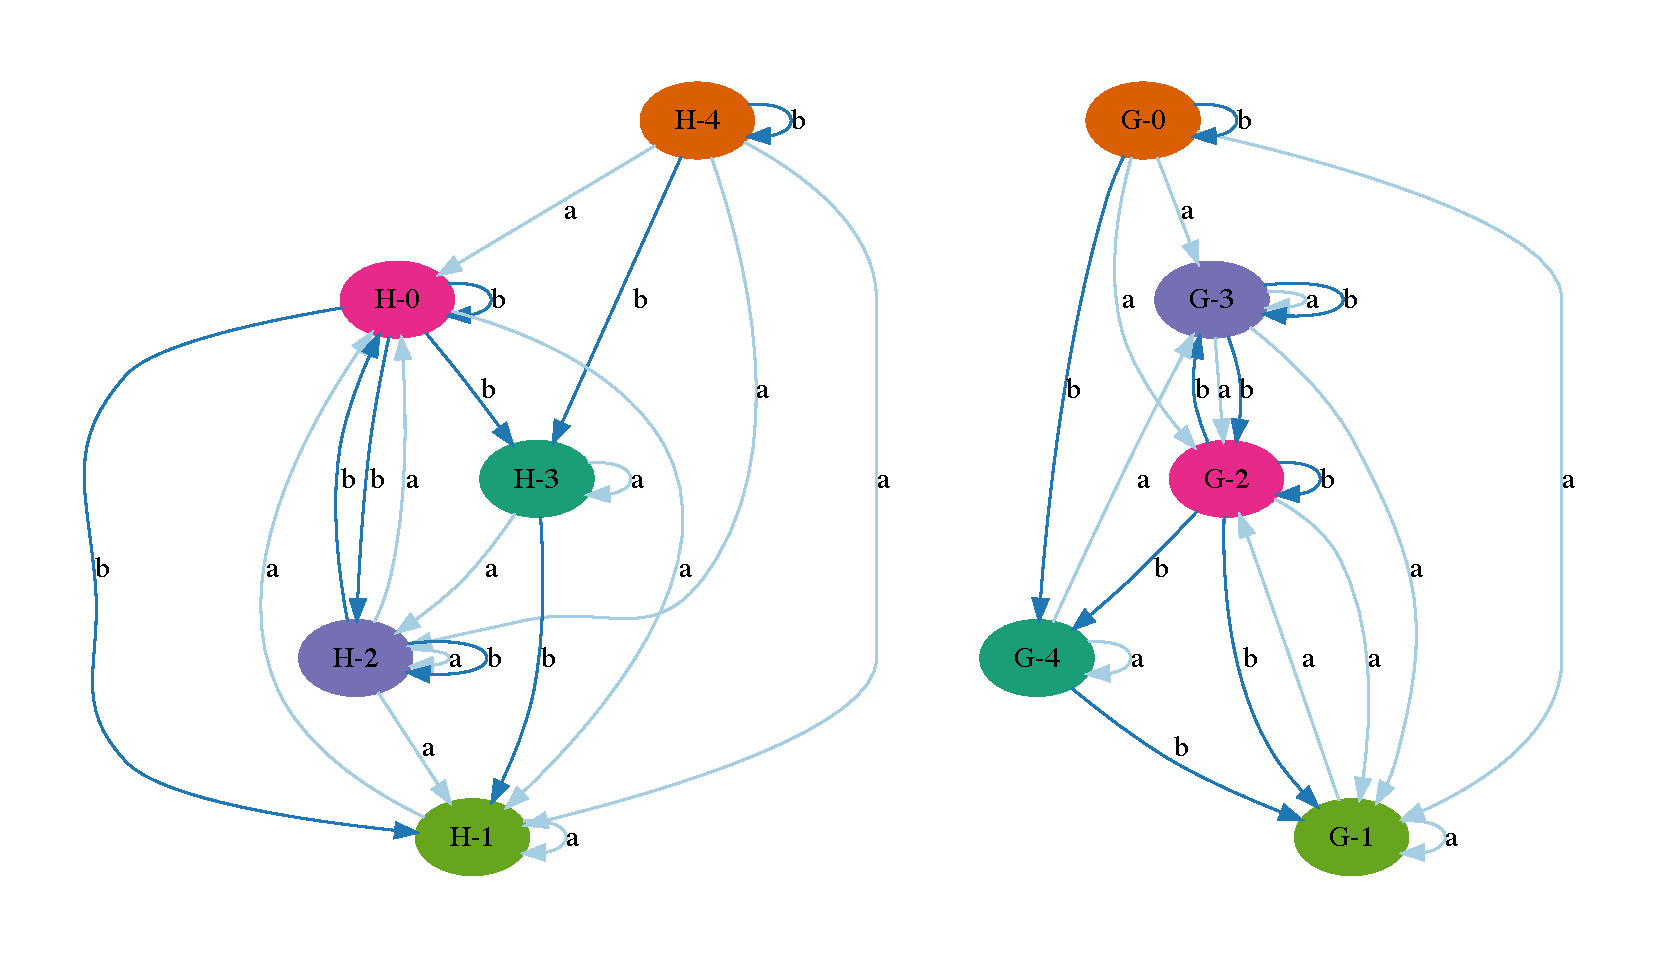
\includegraphics[height=15em]{img/outputg3.pdf}}
    \caption{Test result 3}
    \label{fig:outputg3}
\end{figure}

\begin{figure}[H]
    \centering
    \subfigure[Mini graph]{
        % \label{fig:example1_model}
        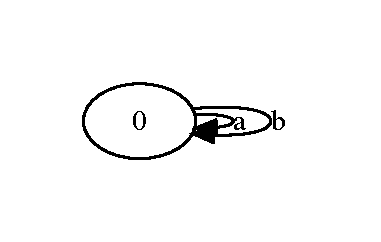
\includegraphics[height=4em]{img/outputg4m.pdf}}
    \subfigure[Coloured graphs]{
        % \label{fig:example1_matrix}
        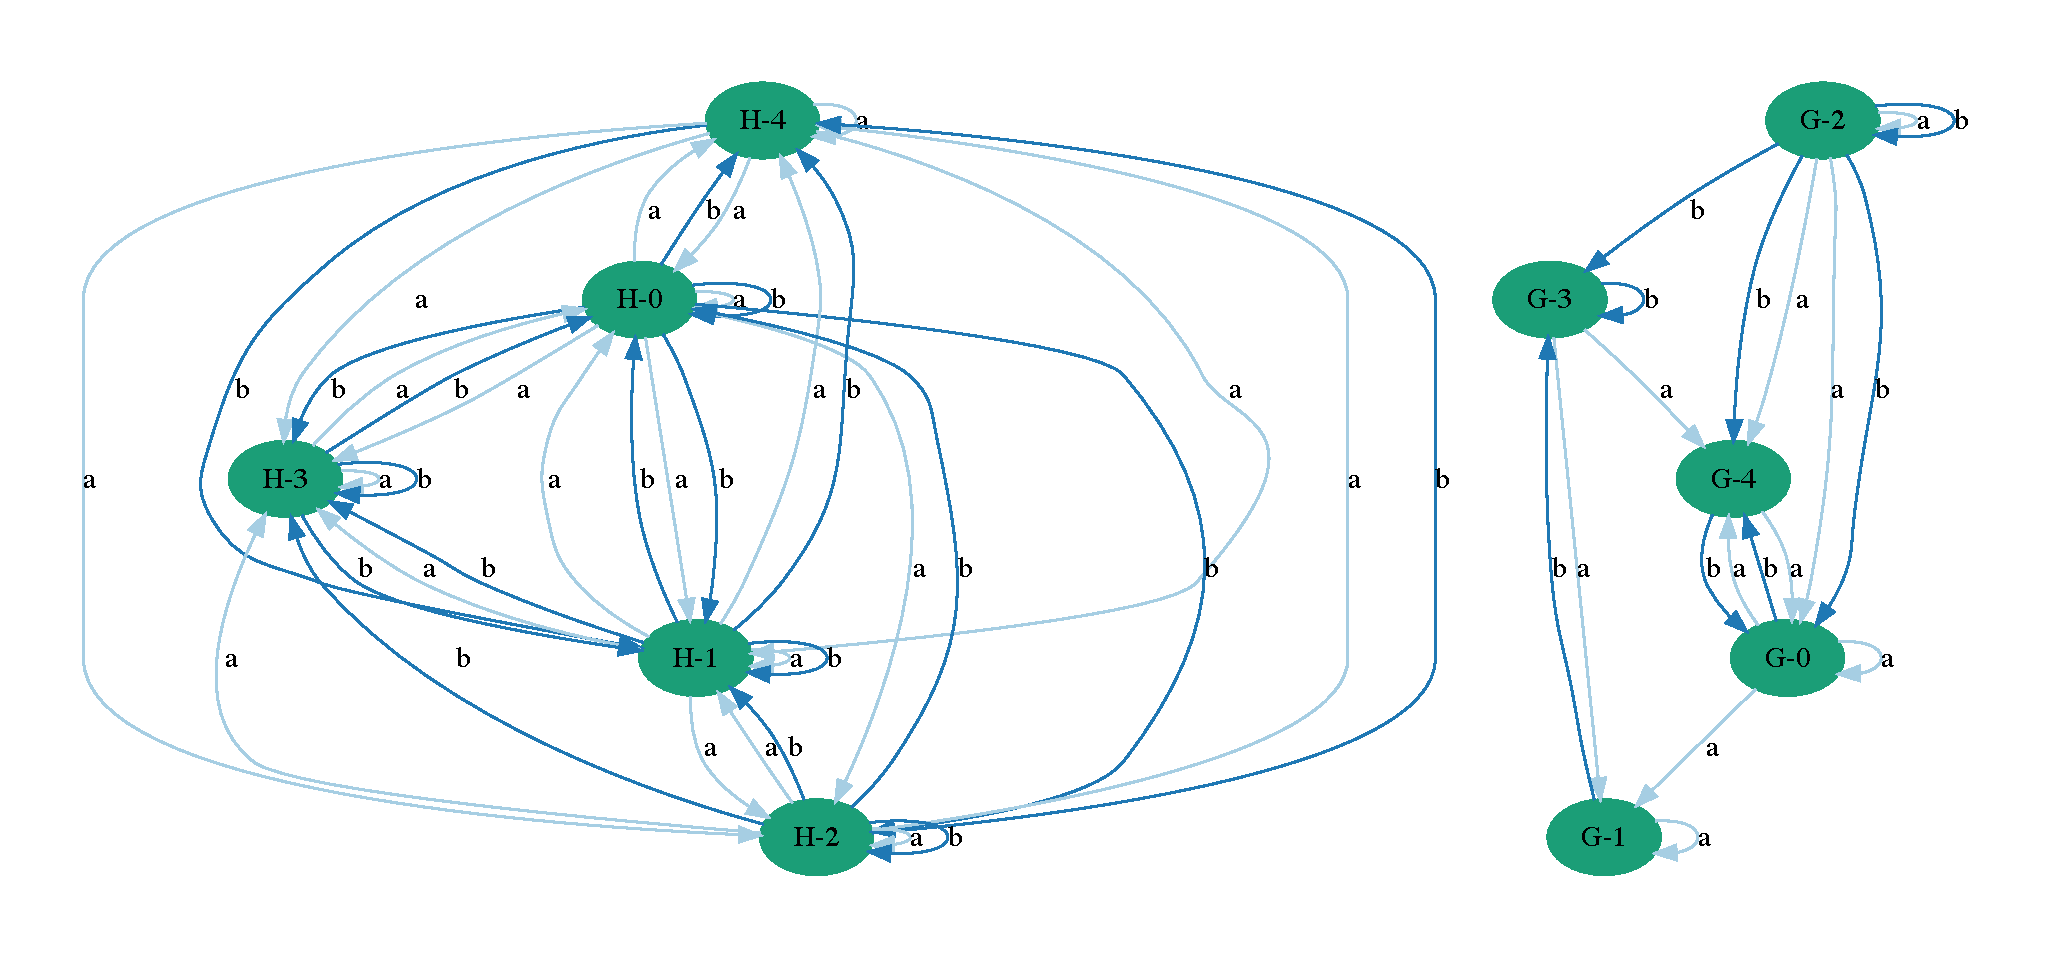
\includegraphics[height=14.5em]{img/outputg4.pdf}}
    \caption{Test result 4}
    \label{fig:outputg4}
\end{figure}


\noindent\textbf{Functions for generator:}
\noindent For the Generator, the test is for the I/O.
Here part of the file generated with 3 nodes and 2 types of edge is given in Table \ref{tab:partoffile}. 
And the running time screenshot is shown in Figure \ref{fig:runscreengen}.

\begin{figure}[h]
\centering
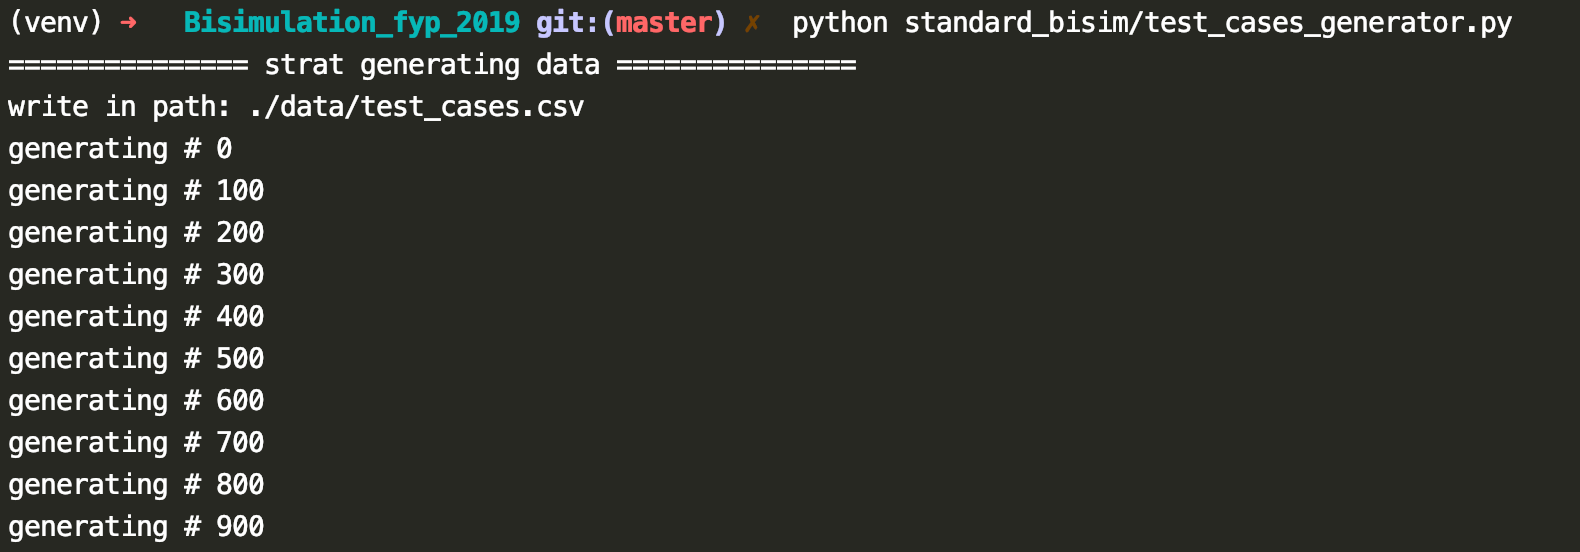
\includegraphics[width=\textwidth]{img/runscreengen.png}
\caption{Screen shot of generator running}
\label{fig:runscreengen}
\end{figure}

\begin{table}[h]
\small
\centering
\begin{tabular}{ |c|c|c| } 
 \hline
    g1 & g2 & bis \\
 \hline
    1, 1, 1, 1, 0, 1, 1, 0, 0, 0, 1, 1, 0, 1, 1, 1, 0, 1  &  0, 0, 0, 0, 0, 0, 1, 1, 0, 1, 0, 1, 1, 0, 0, 1, 1, 0  &  0 \\
    0, 1, 0, 0, 0, 0, 0, 1, 0, 1, 0, 0, 1, 0, 1, 0, 0, 0  &  0, 0, 1, 0, 1, 0, 0, 0, 0, 1, 0, 1, 0, 0, 0, 1, 0, 1  &  1 \\
    1, 0, 0, 1, 0, 0, 0, 0, 0, 1, 0, 0, 0, 1, 1, 0, 1, 0  &  0, 1, 0, 0, 0, 0, 0, 1, 1, 0, 0, 0, 1, 0, 0, 1, 1, 0  &  1 \\
    0, 0, 0, 0, 0, 1, 0, 0, 0, 0, 0, 1, 0, 0, 1, 0, 0, 0  &  1, 1, 1, 0, 1, 1, 0, 0, 0, 1, 0, 1, 1, 1, 0, 0, 0, 0  &  0 \\
    1, 0, 0, 1, 0, 0, 0, 0, 0, 0, 0, 0, 1, 1, 1, 0, 1, 1  &  0, 0, 1, 1, 0, 0, 0, 1, 1, 1, 1, 0, 1, 1, 1, 0, 1, 1  &  0 \\
    1, 0, 0, 0, 0, 0, 1, 0, 0, 0, 0, 0, 0, 0, 0, 1, 0, 0  &  0, 0, 1, 0, 0, 1, 0, 0, 0, 0, 0, 0, 0, 0, 0, 0, 0, 1  &  0 \\
    1, 0, 0, 0, 1, 1, 1, 1, 0, 0, 0, 0, 0, 1, 0, 0, 0, 0  &  0, 1, 0, 1, 1, 1, 1, 1, 1, 1, 1, 1, 0, 0, 1, 1, 0, 1  &  0 \\
    1, 1, 1, 1, 0, 0, 1, 0, 0, 0, 1, 0, 0, 1, 0, 1, 1, 0  &  1, 0, 0, 1, 0, 1, 0, 0, 1, 1, 1, 1, 1, 0, 1, 0, 0, 0  &  1 \\
    0, 1, 0, 1, 0, 0, 1, 0, 1, 1, 0, 0, 1, 1, 0, 0, 1, 1  &  0, 0, 0, 1, 0, 1, 1, 1, 1, 0, 1, 1, 1, 0, 1, 0, 0, 0  &  0 \\
    1, 1, 1, 0, 1, 0, 1, 1, 1, 1, 1, 1, 0, 1, 1, 0, 0, 1  &  1, 1, 1, 0, 1, 0, 1, 1, 1, 0, 1, 1, 1, 1, 1, 1, 1, 1  &  1 \\
    ...  & ...  & ... \\
 \hline
\end{tabular}
\caption{Part of the generated file \texttt{test\char`_cases.csv}}
\label{tab:partoffile}
\end{table}



\subsubsection{Test for ML Algorithm}
Here we will use some simple generated test cases.
And through the change of the metrics, the algorithm can be tested on some level.
Here give graphs of first 1000 epochs training of the test sample where the node number is 3 and the type number of edges is 2 and 1000 entries (see Figure \ref{fig:mlt1}), along with the running time screenshot (see Figure \ref{fig:runscreenml}).
The orange and blue lines indicate the trend of metrics on train data and test data respectively.
In Figure \ref{fig:mlt1acc}, along with the training the accuracy on training data and test data growth distinctively.
And in Figure \ref{fig:mlt1loss}, the loss on both data sets decreases.
Several tests show similar results.
It denotes that the model is actually learning as expected.

\begin{figure}[h]
\centering
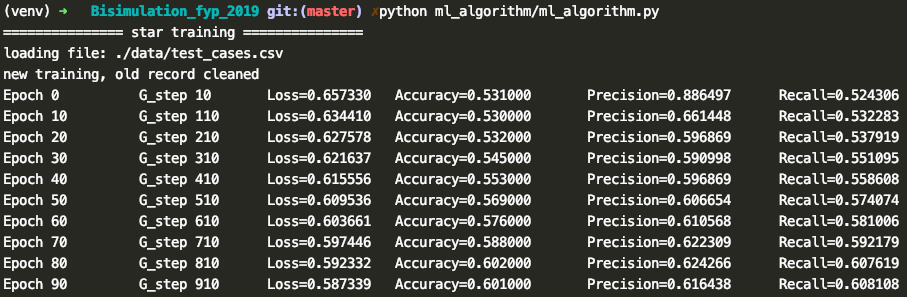
\includegraphics[width=\textwidth]{img/runscreenml.png}
\caption{Screen shot of machine learning algorithm running}
\label{fig:runscreenml}
\end{figure}

\begin{figure}[h]
    \centering
    \subfigure[Accuracy]{
        \label{fig:mlt1acc}
        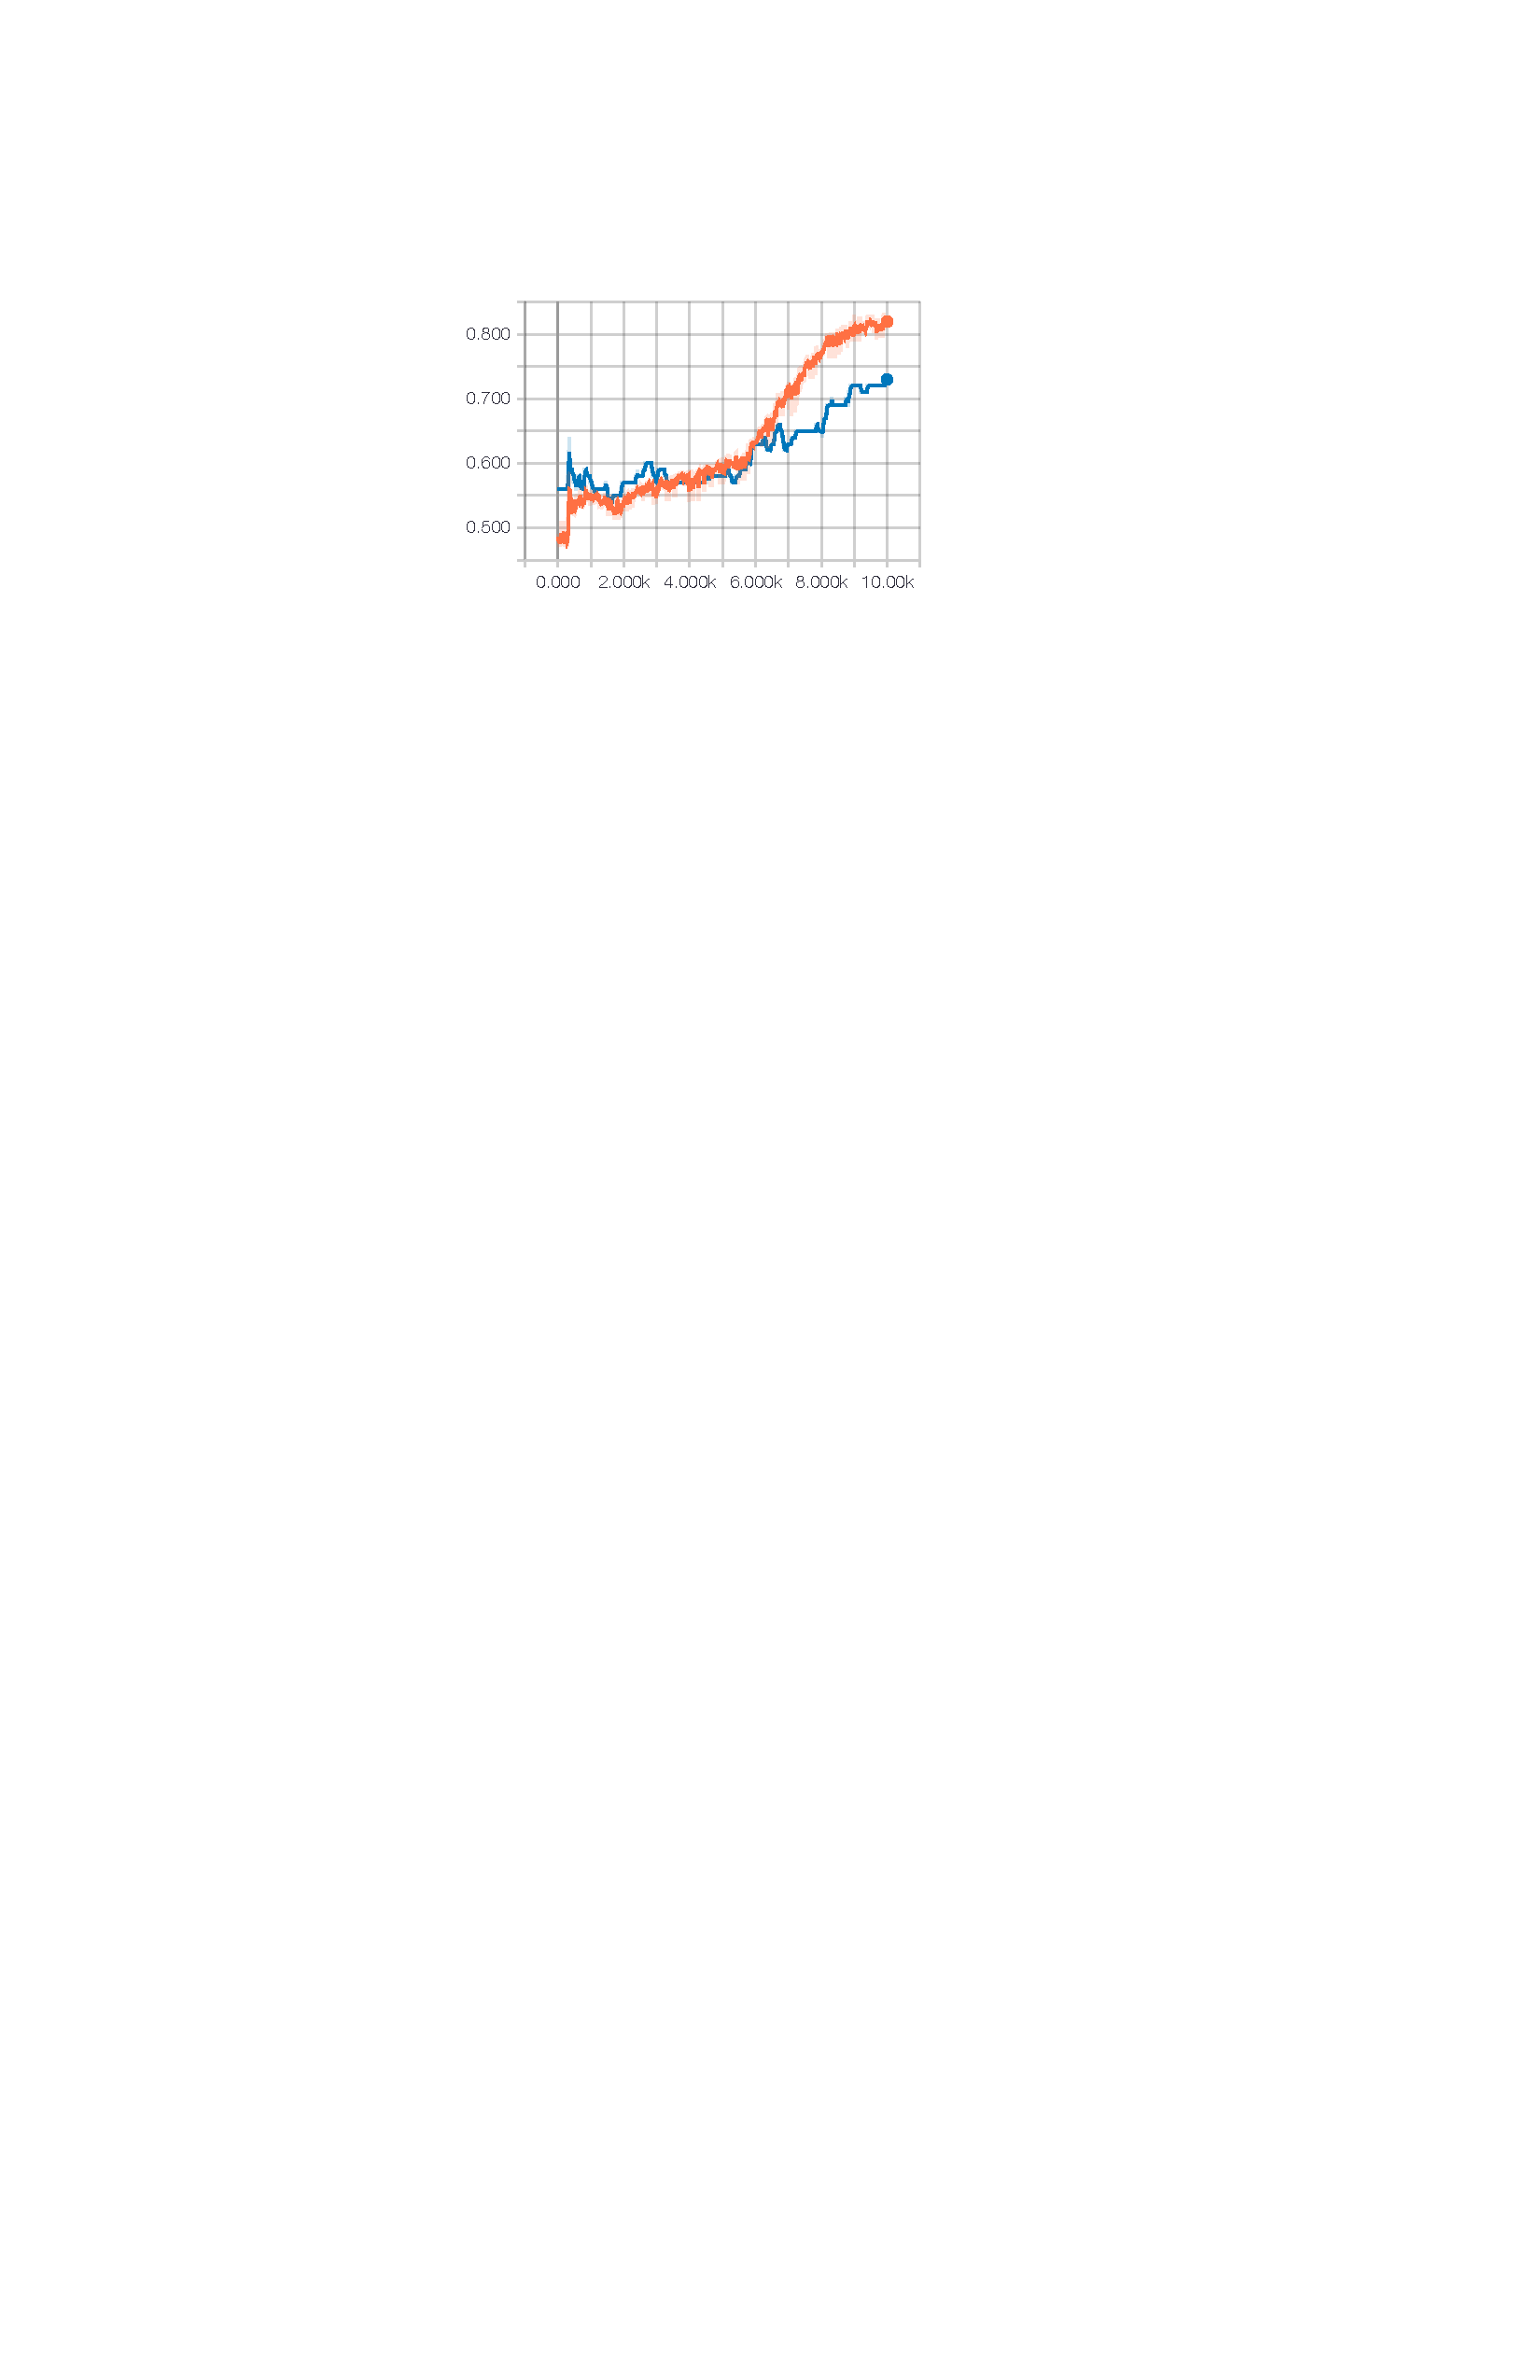
\includegraphics[width=0.45\textwidth]{img/mlaccuracyt1.pdf}}
        % \includesvg[width=0.45\textwidth]{img/accuracy.svg}}
    \subfigure[Loss]{
        \label{fig:mlt1loss}
        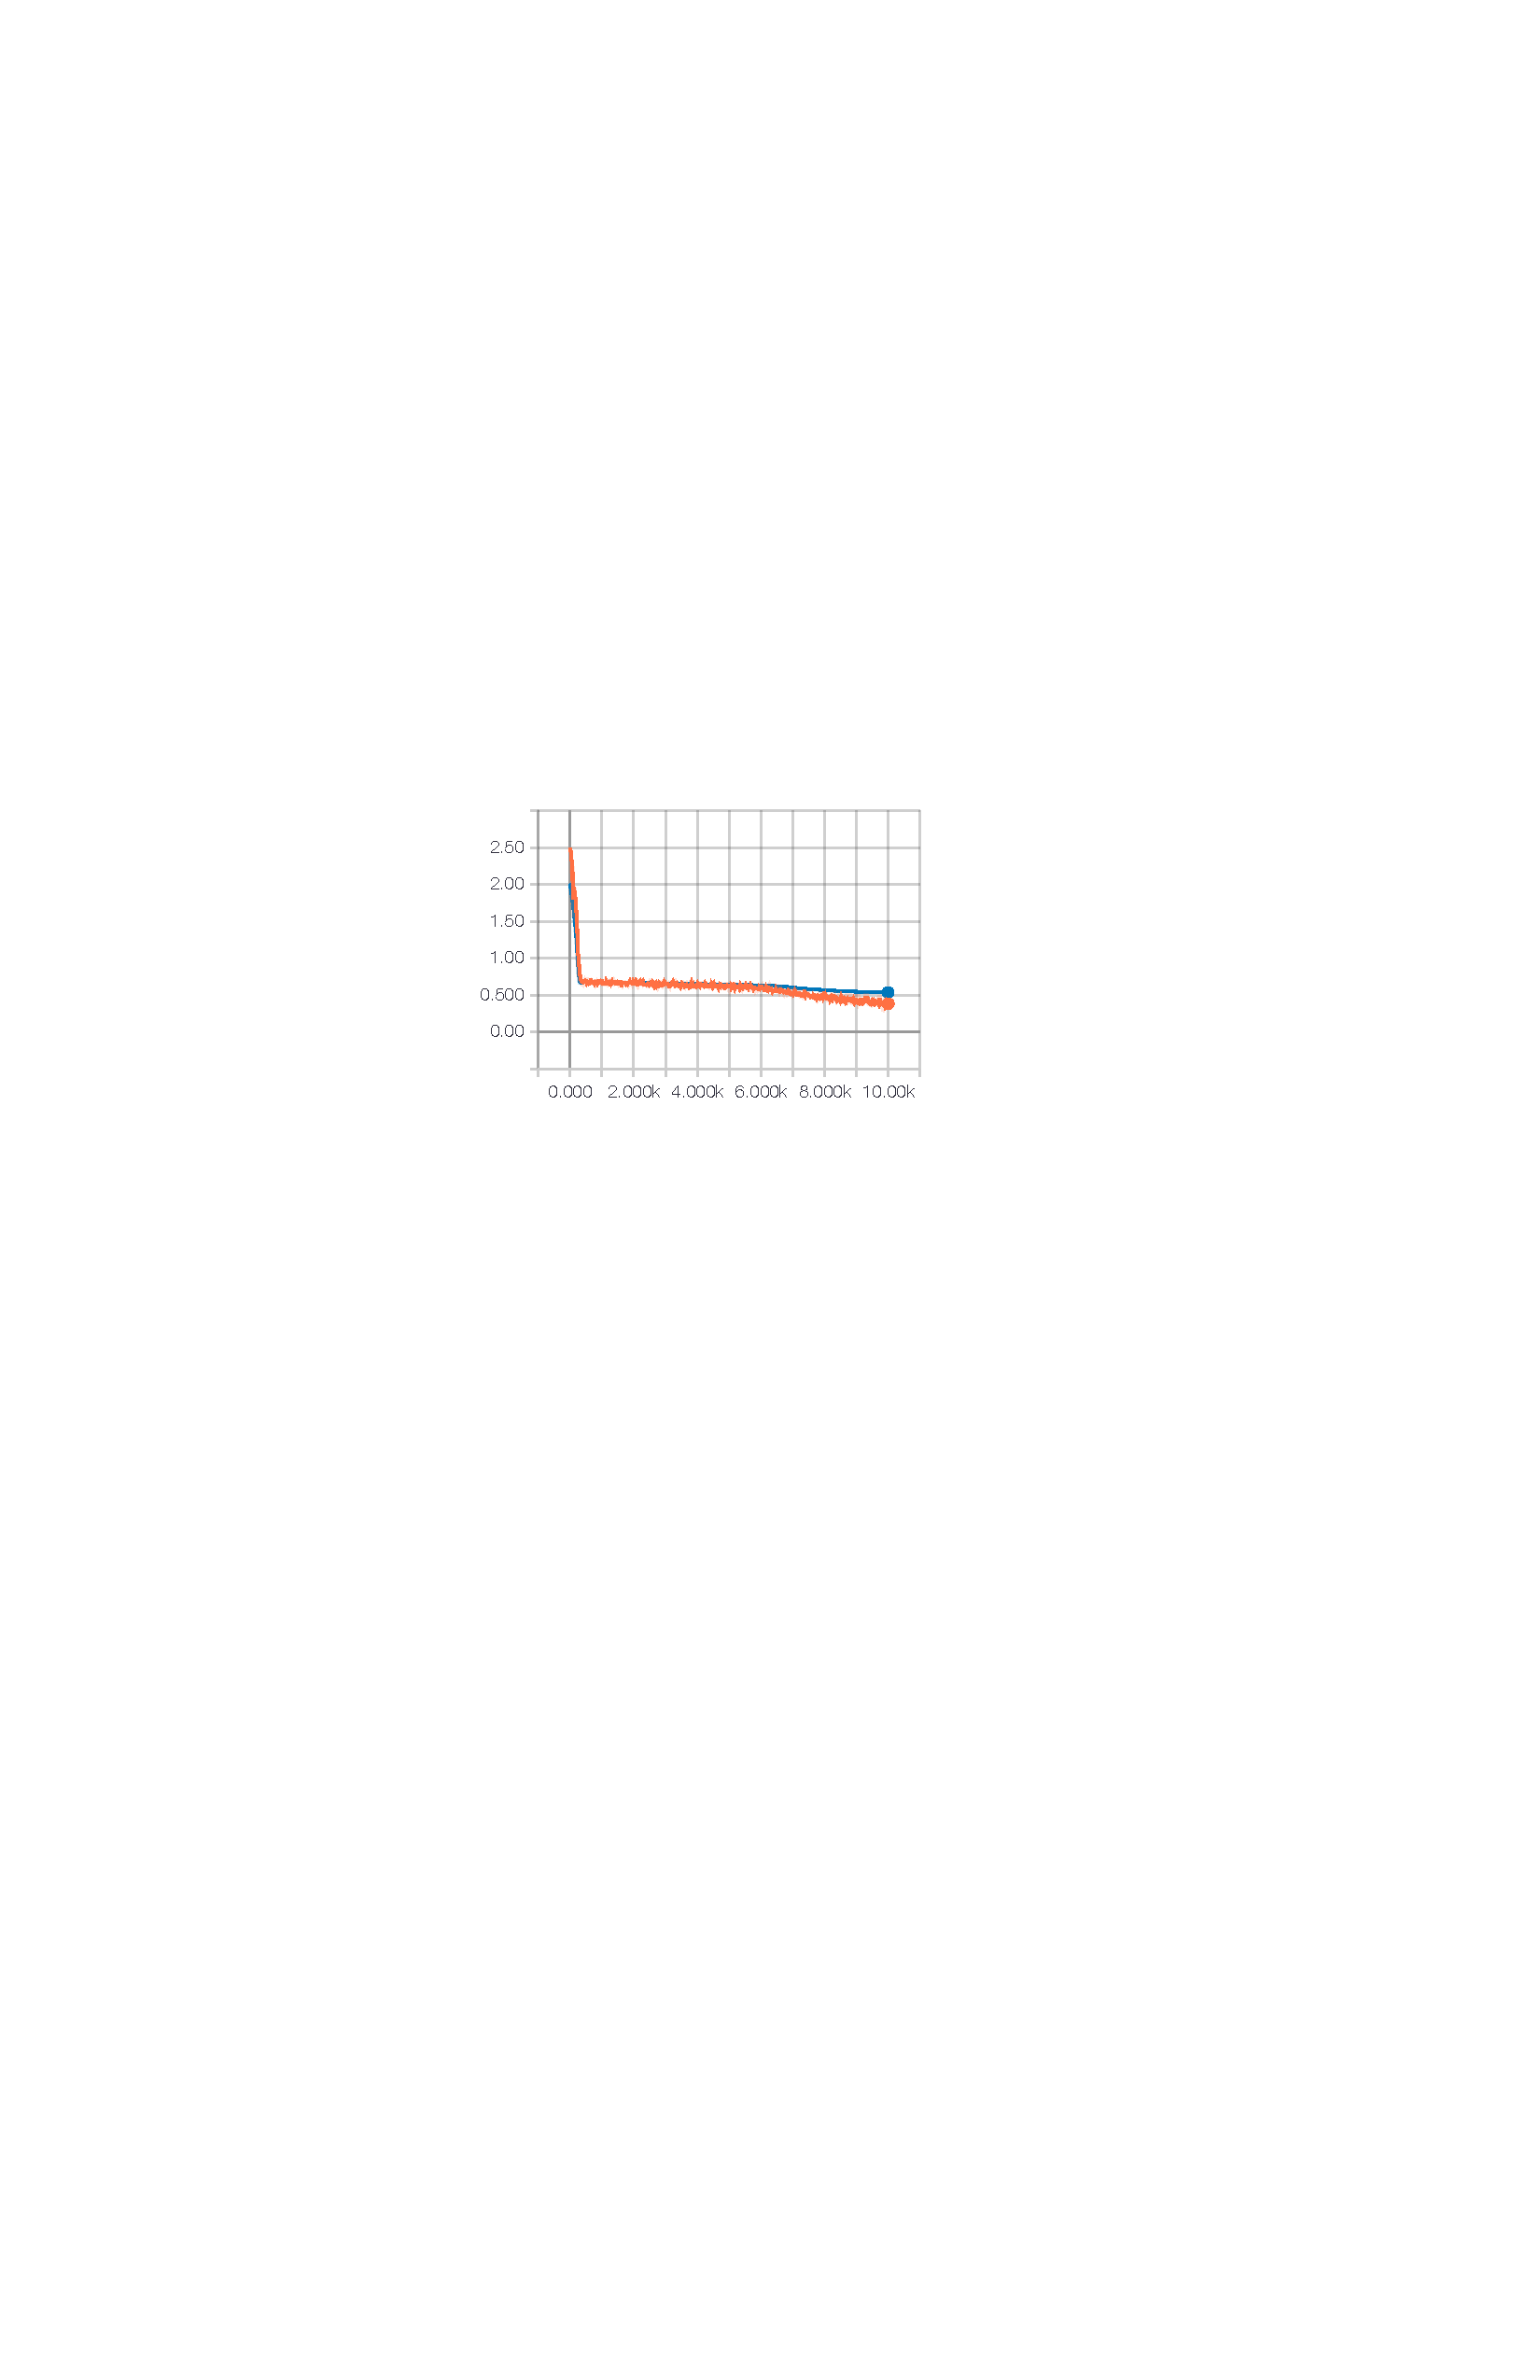
\includegraphics[width=0.45\textwidth]{img/mllosst1.pdf}}\\
    \subfigure[Precision]{
        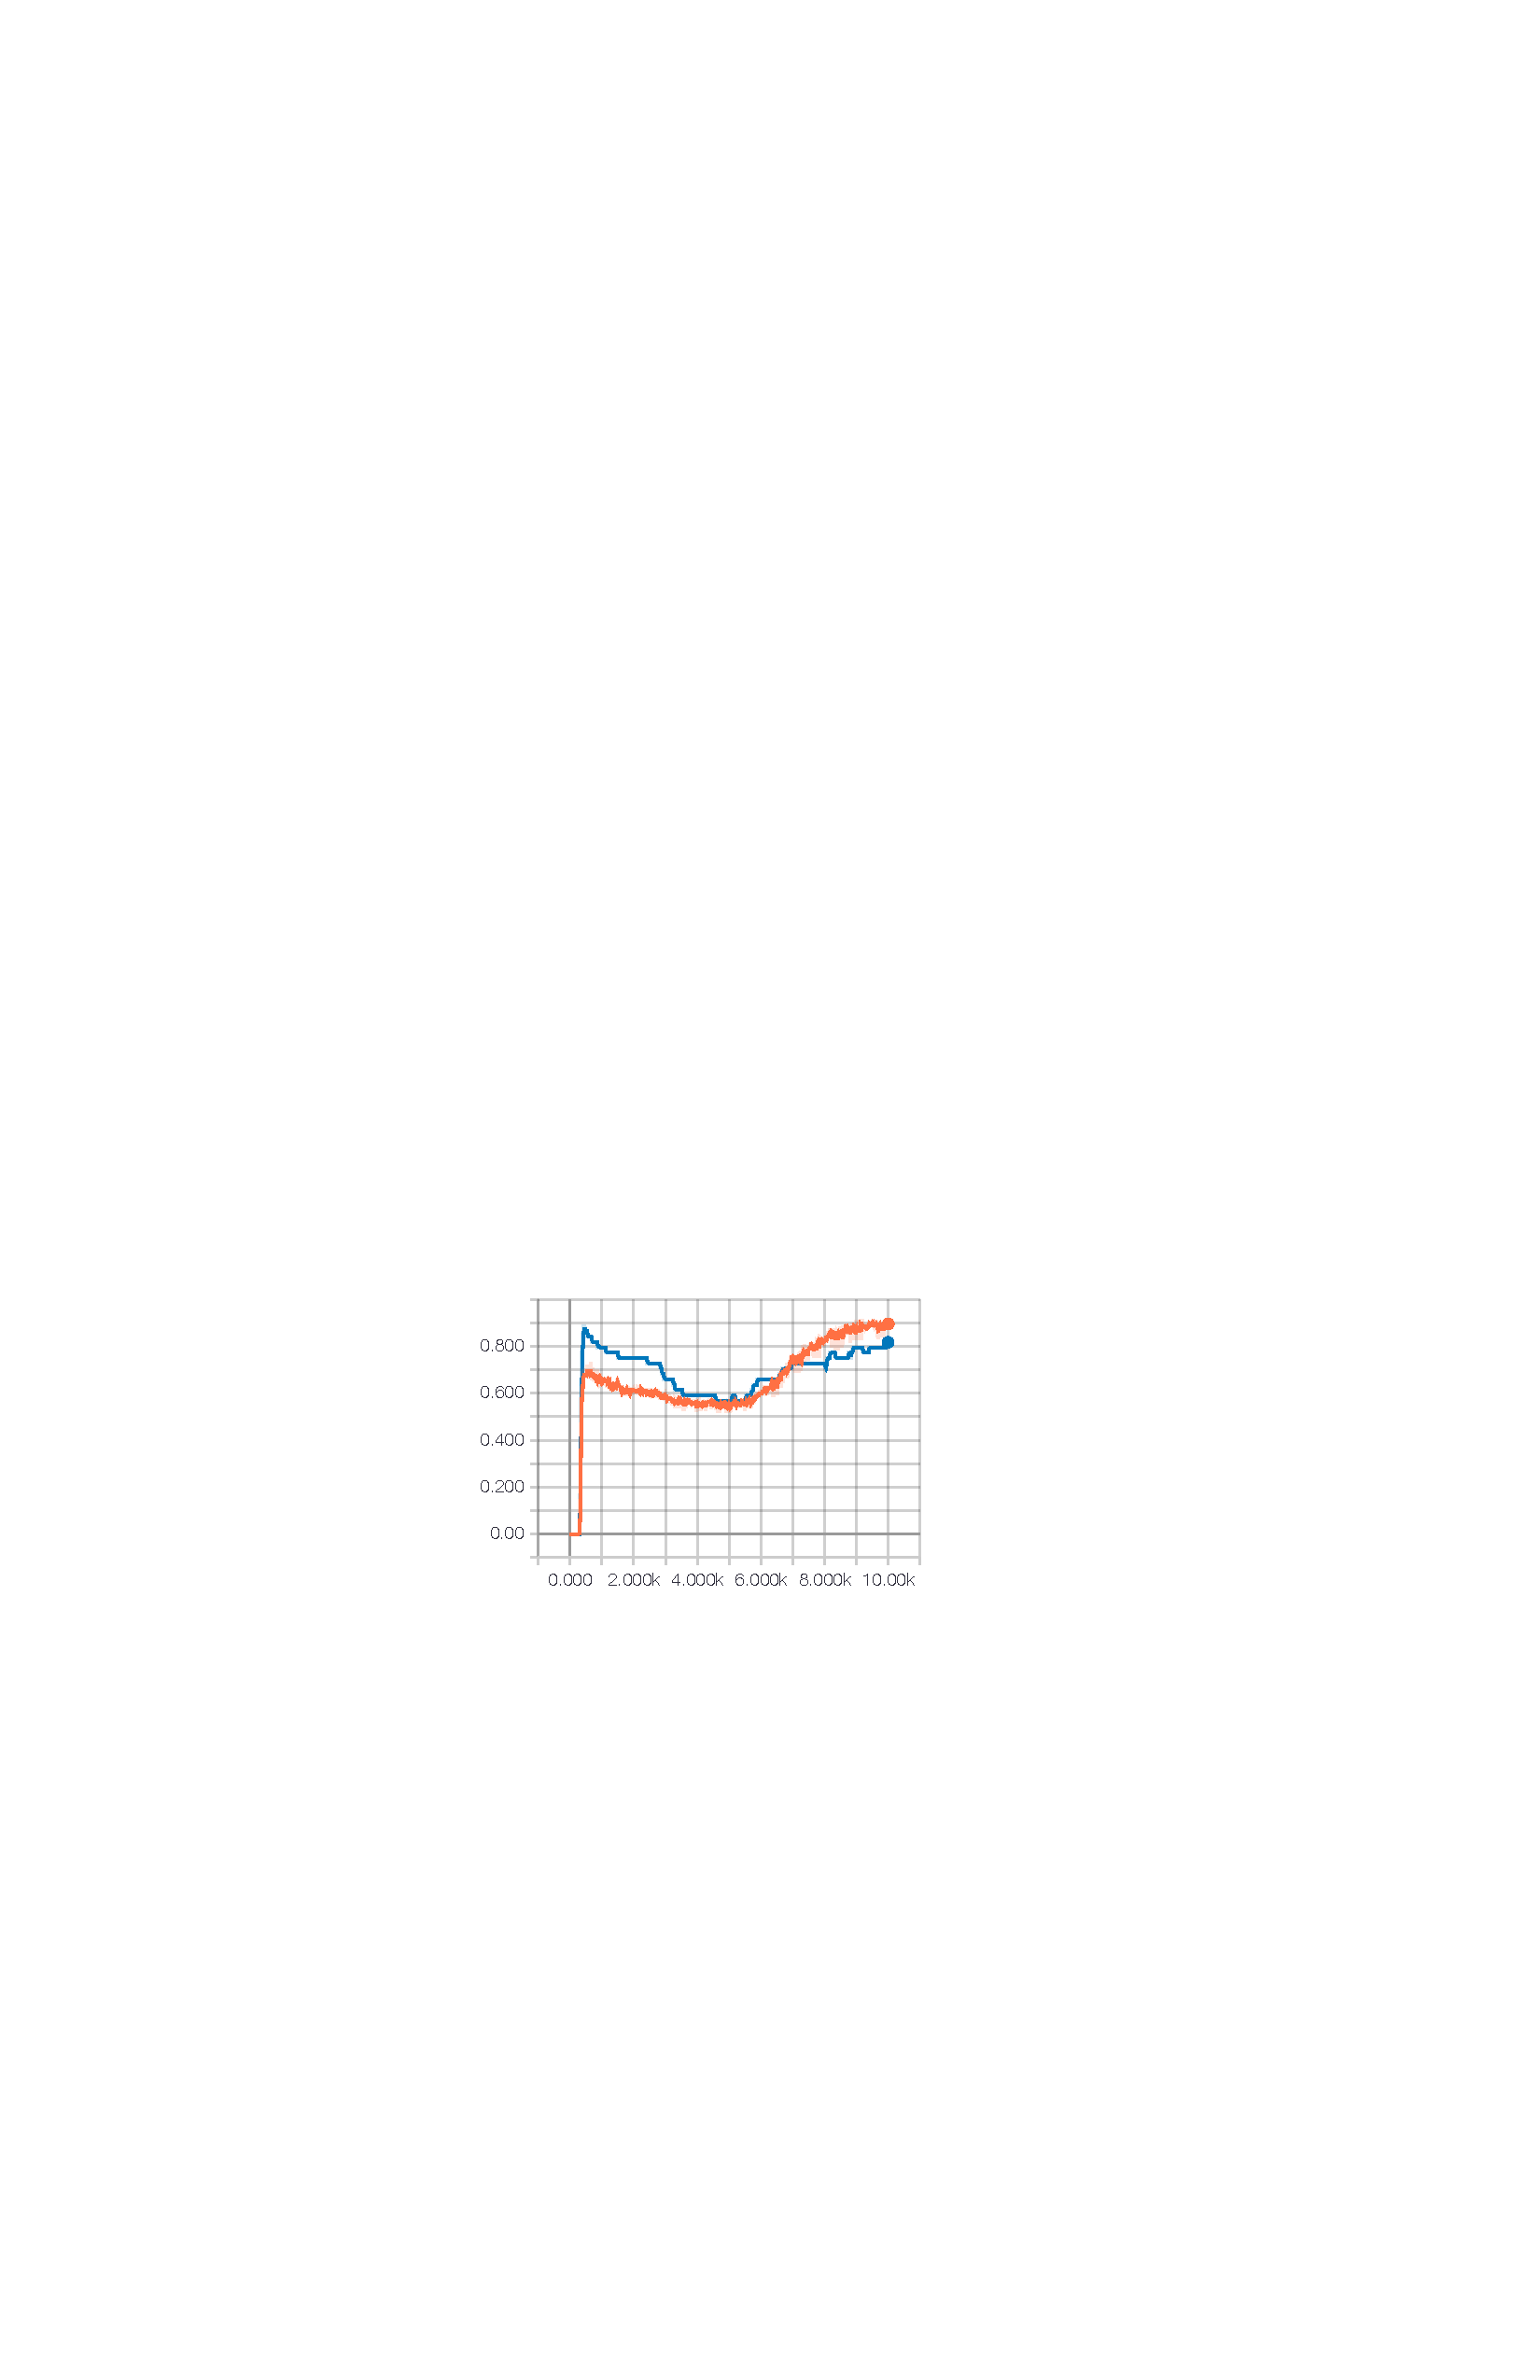
\includegraphics[width=0.45\textwidth]{img/mlprecisiont1.pdf}}
    \subfigure[Recall]{
        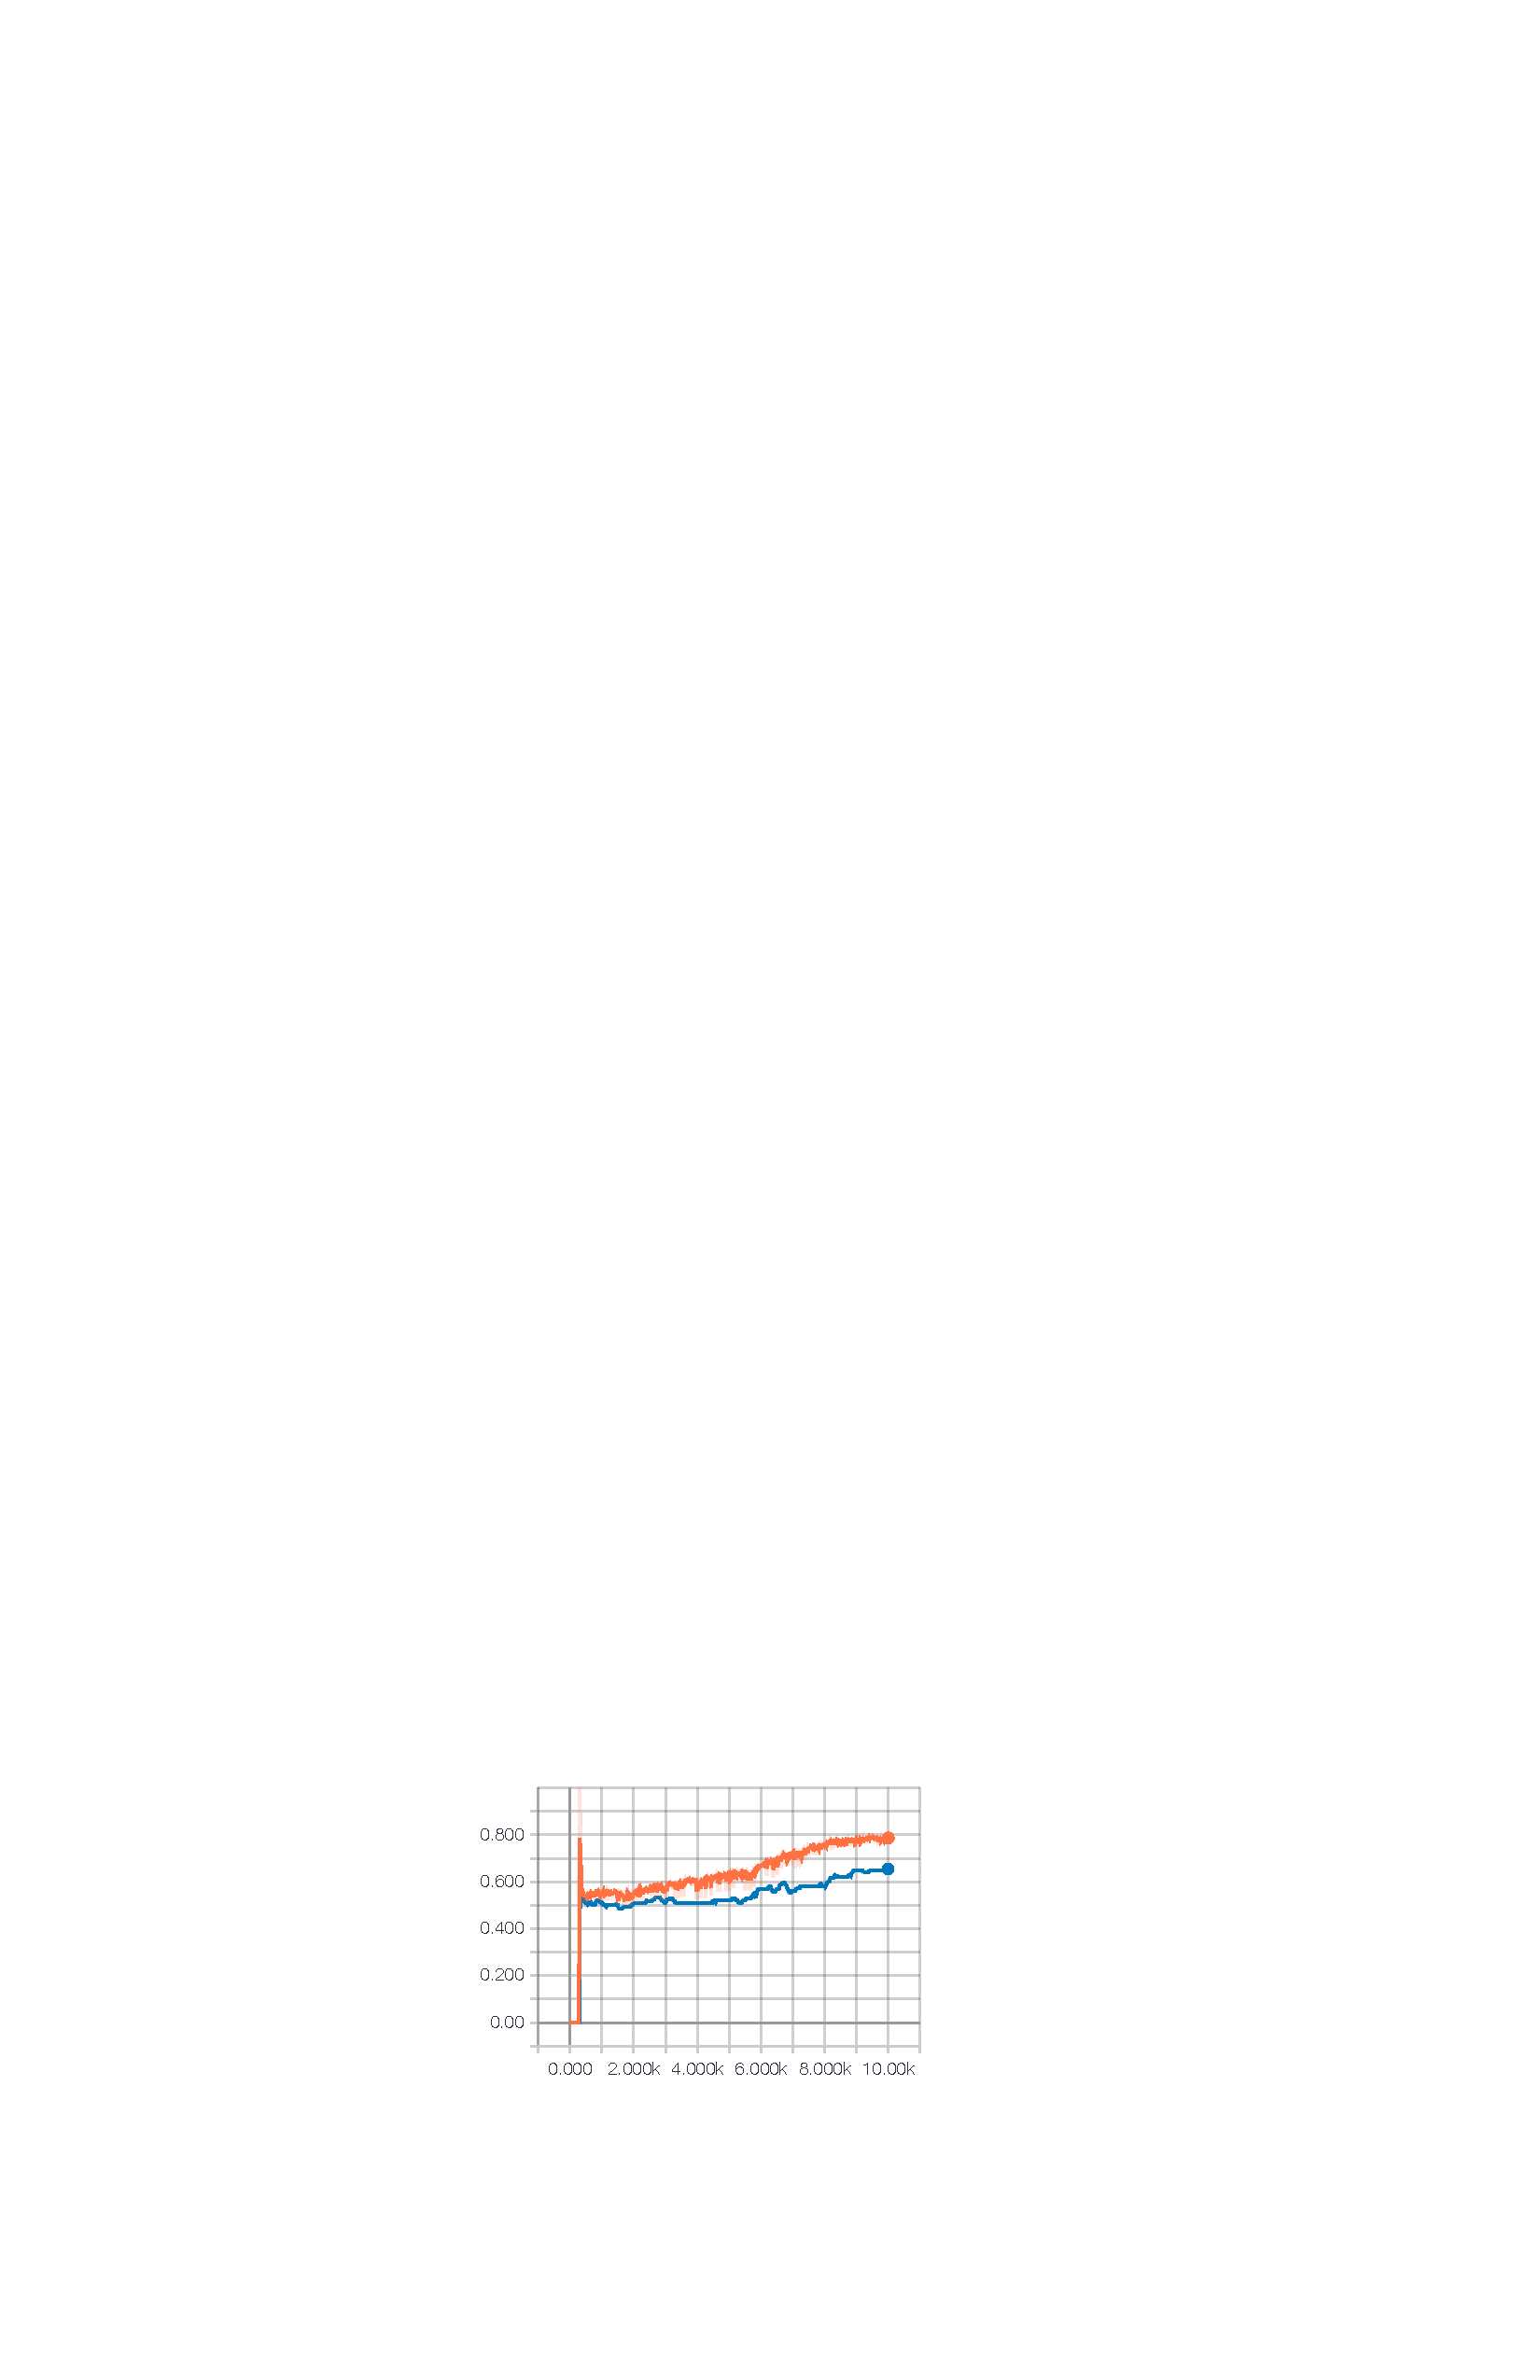
\includegraphics[width=0.45\textwidth]{img/mlrecallt1.pdf}}
    \caption{Metrics for test training sample}
    \label{fig:mlt1}
\end{figure}


\subsection{Project Progress}
The whole project is mainly divided into three parts.
Each phase took around 2 months.
The first part is concentrated on the literature review and prepare the knowledge about machine learning (detail will be included in Section \ref{sec:learning}).
\begin{itemize}
    \item Literature review about bisimulation
    \item Literature review about machine learning on logic
    \item Learn to use packages
    \item Plan and design the project
\end{itemize}
The second part is to develop a bisimulation algorithm and a test cases generator.
\begin{itemize}
    \item Review relevant work on bisimulation
    \item Implement the standard algorithm
    \item Develop the visualisation tool
    \item Test and adjust the developed algorithm
    \item Develop the test case generator 
    \item Test and adjust the generator 
\end{itemize}
The last part is to construct the machine learning algorithm and experiment.
\begin{itemize}
    \item Review relevant work on the logical learning in neural network 
    \item Learn to use TensorFlow 
    \item Implement the neural network 
    \item Test the network and adjust the hyper-parameters
    \item Experiment on different cases (to be seen in Section \ref{sec:experiment})
\end{itemize}
For the timeline of the project, Gantt-chart is given below in Figure \ref{fig:ganttchart}.

\begin{figure}[hp]
    \centering
    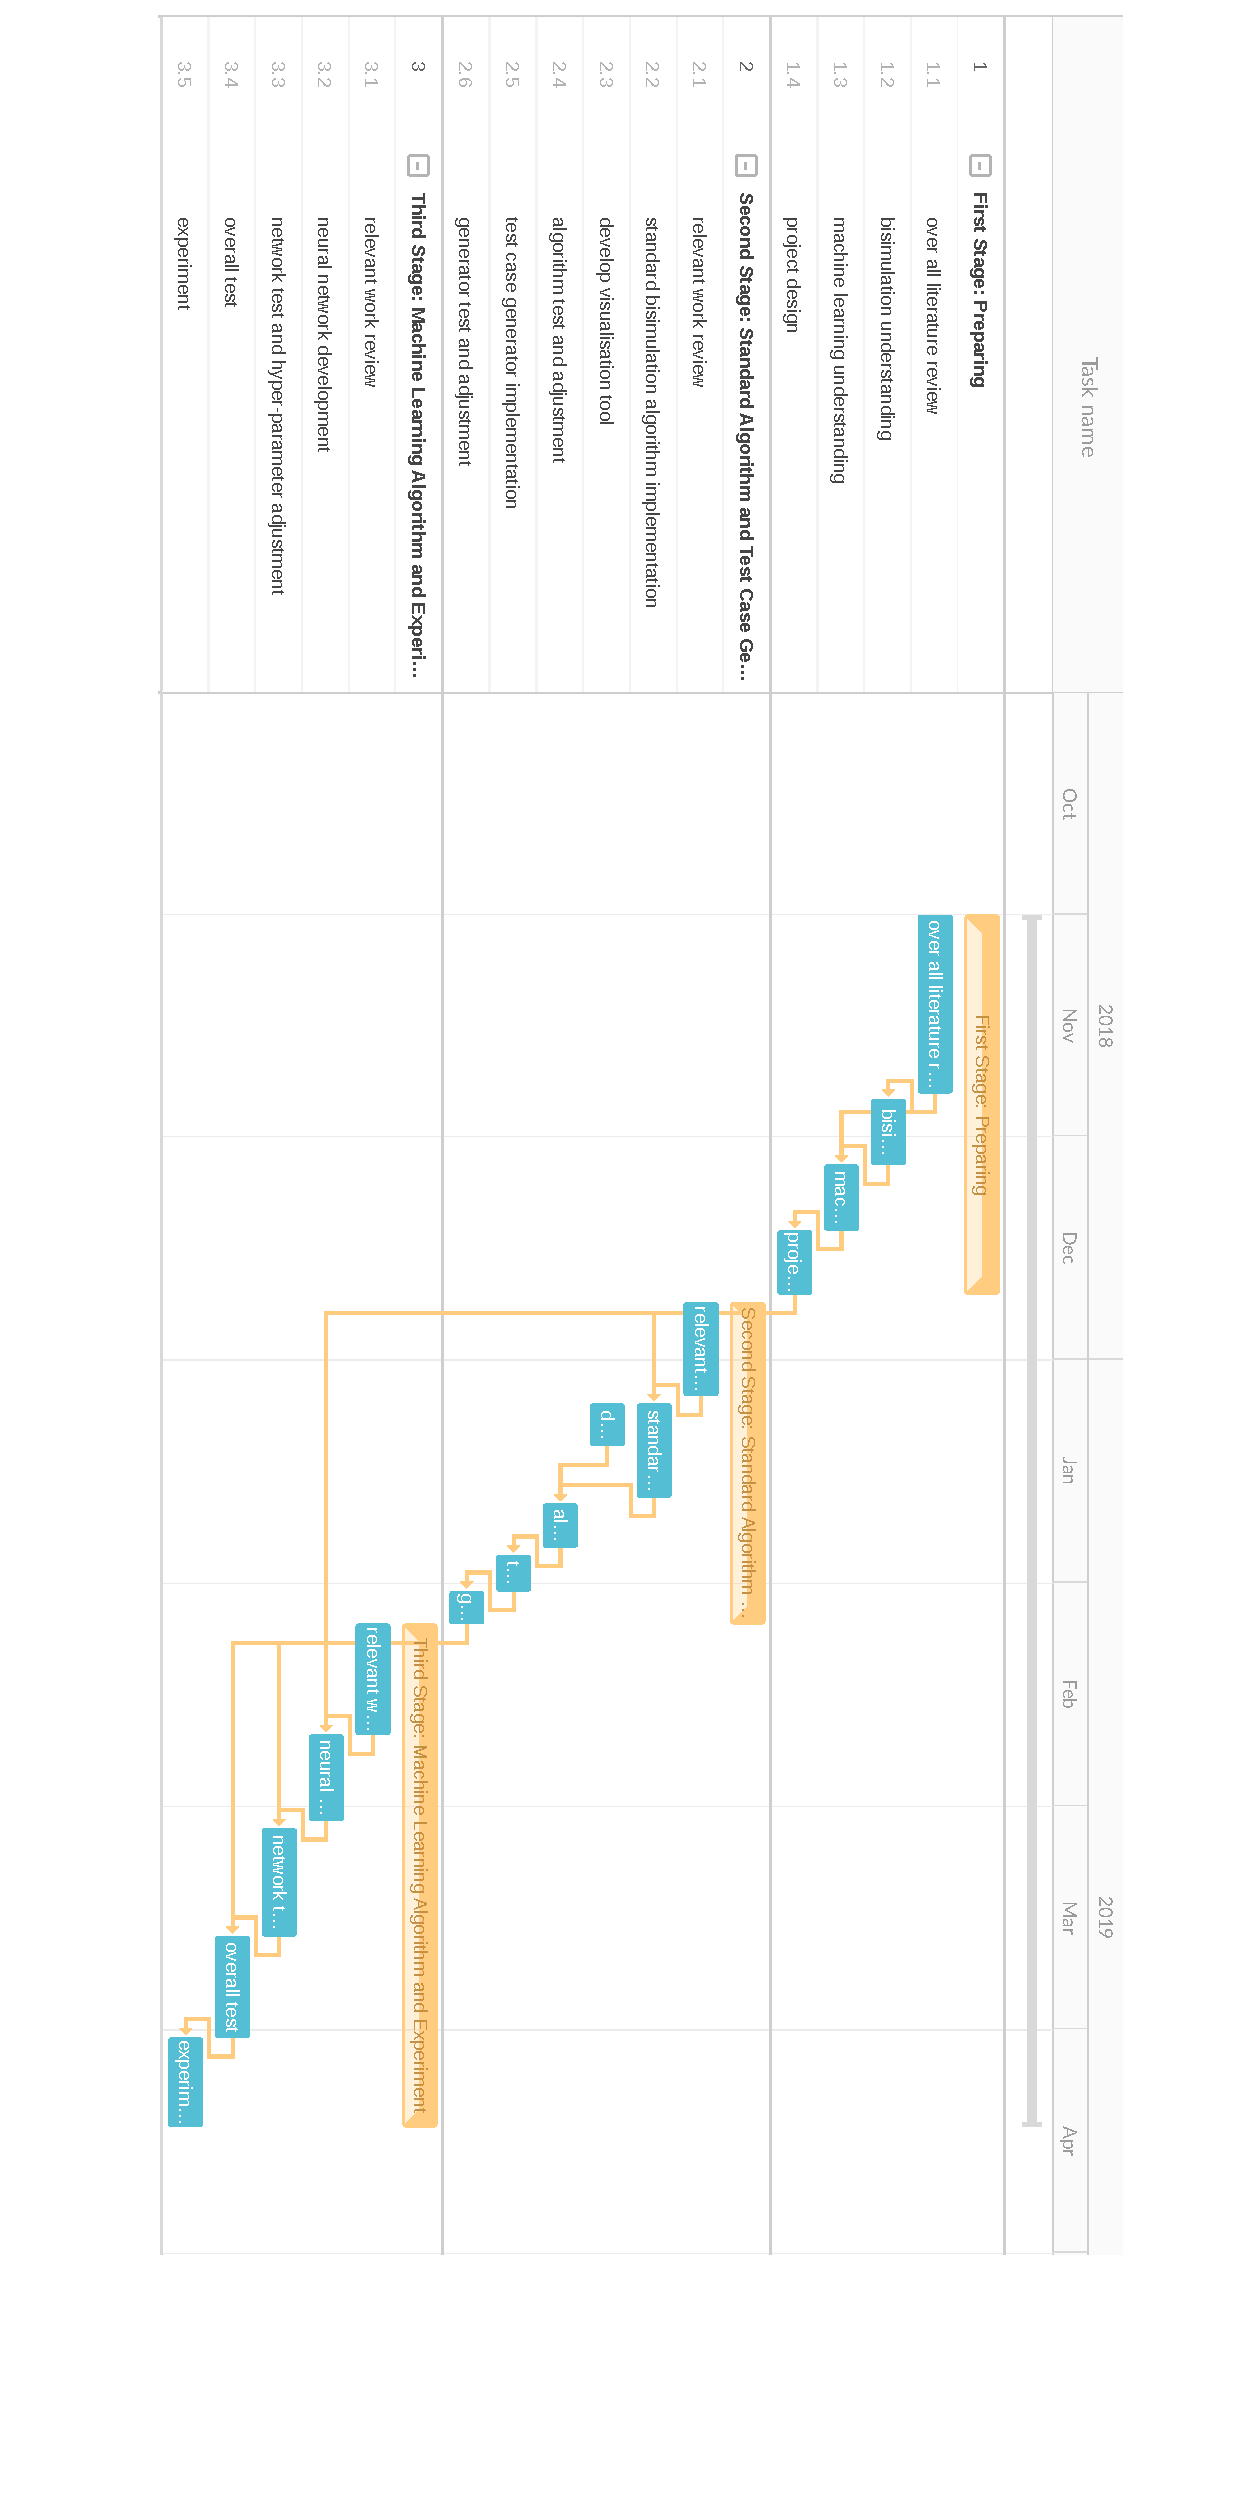
\includegraphics[height=\textheight]{img/gantt.pdf}
    \caption{Gantt Chart}
    \label{fig:ganttchart}
\end{figure}






\subsection{Environment}
\subsubsection*{Hardware}
2012 Mac mini computer, with processor Core i5 (i5-3210M), 8GB RAM is used during the developing of the project.
When comes to the experiment, it is run on the Google Cloud Platform with 2 standard vCPUs (virtual CPU), 7.5 GB RAM and one NVIDIA Tesla K80 GPU.
\subsubsection*{Software}
This project is developed on \texttt{PyCharm 2018.3.6}, under \texttt{macOS Mojave 10.14}.
For the main packages/library used in the project, \texttt{NetworkX 2.2} is used to manipulate the graph objects.
The visualisation of the graphs is based on \texttt{ Matplotlib 2.2.3}.
Neural network and relevant training is based on the \texttt{TensorFlow 1.12.0} and \texttt{TensorFlow-GPU 1.12.0}.
For the experiment the project is running under \texttt{Ubuntu 16.04.6 LTS}.